\pagenumbering{Roman}

\chapter*{Anhang}

\setcounter{chapter}{7}

\setcounter{figure}{0}

\lhead{Anhang}

\addcontentsline{toc}{chapter}{Anhang}

\cleardoublepage

\begin{figure}[h]
    \addcontentsline{toc}{section}{\protect\numberline{Anhang A}{\hspace{1.2cm}Klassendiagramm}}
    \lhead{Anhang A \hspace{2mm} Klassendiagramm}
    \begin{center}
     %  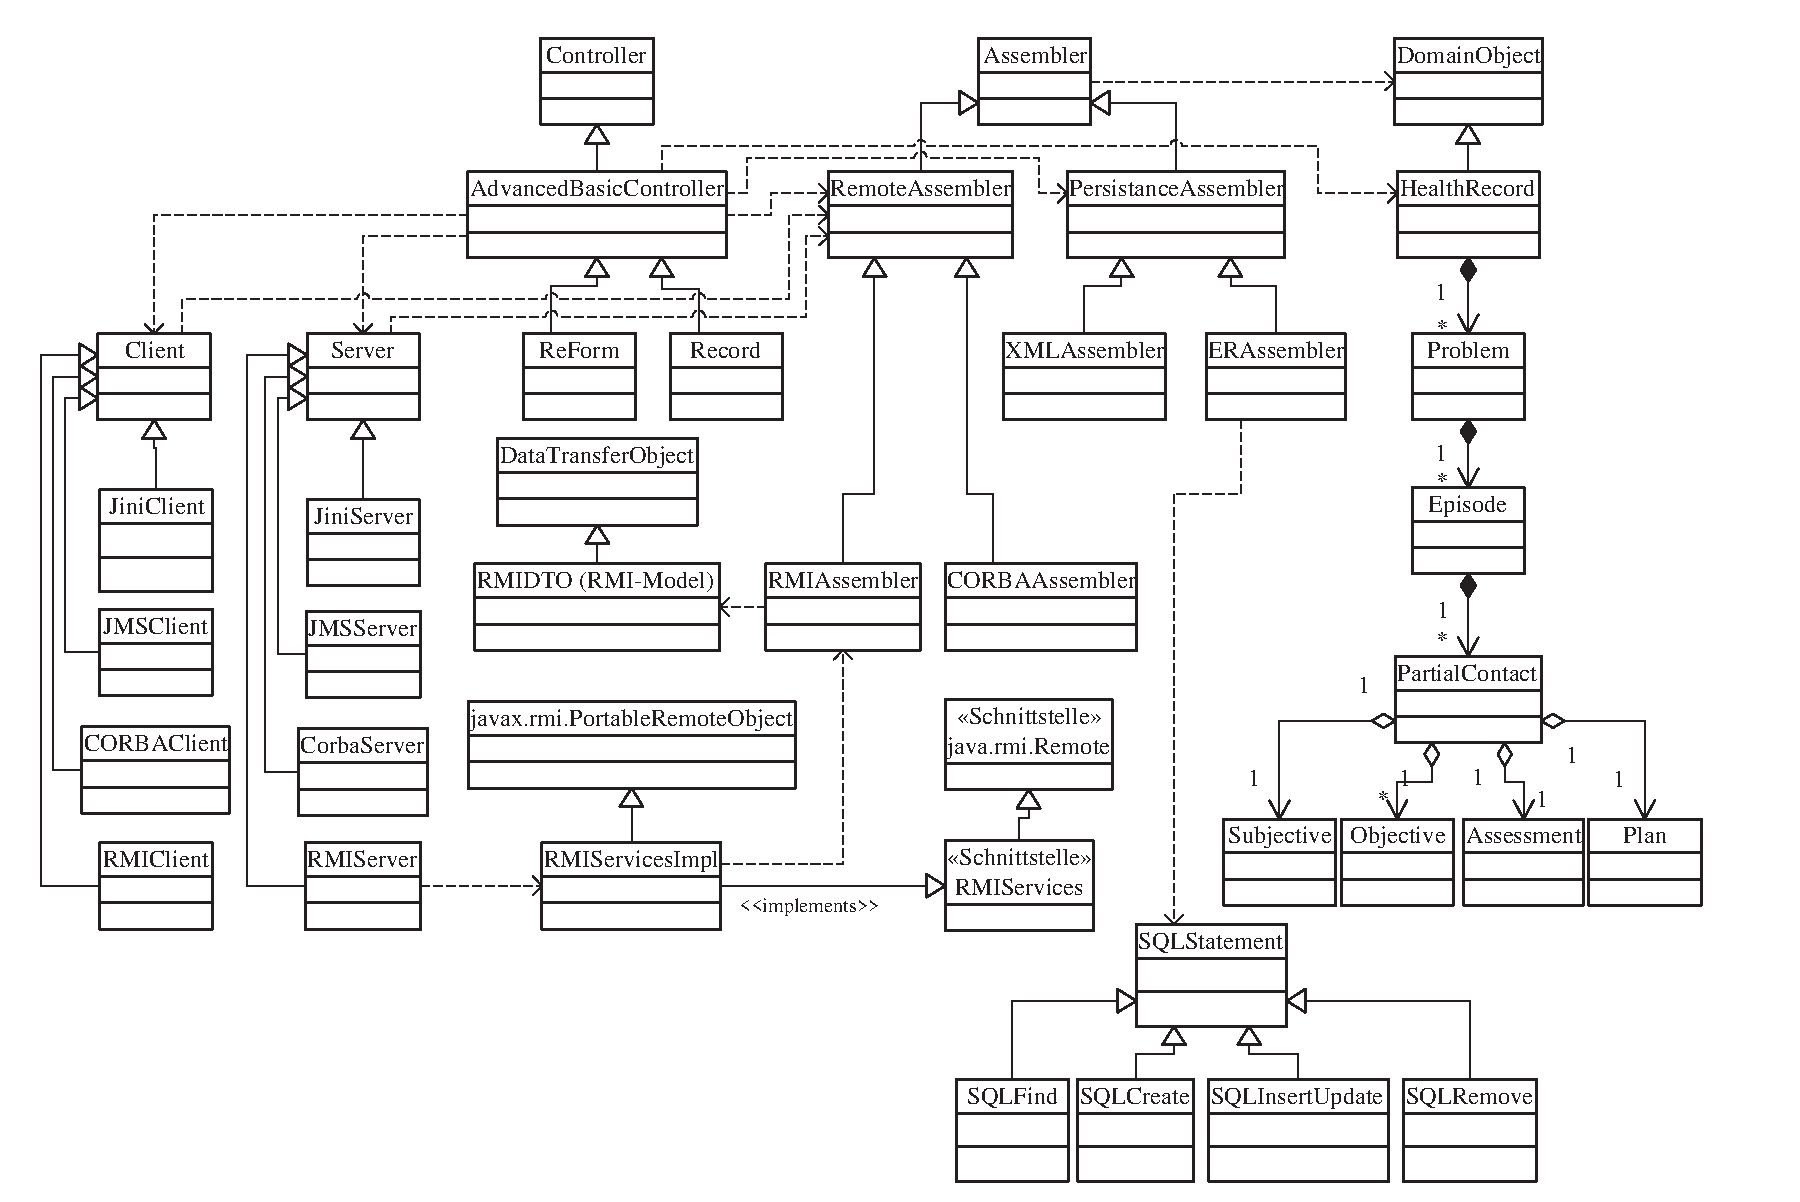
\includegraphics[angle= 90,scale=0.74]{Bilder/GesamtModell.eps}
       \includegraphics[bb=0 0 800 550,angle= 90,scale=0.78]{Bilder/GesamtModell_schattiert.eps}
       \caption{Klassendiagramm der in Kapitel \ref{Die Gesamtarchitektur} und \ref{Das Formularmodul - ReForm} beschriebenen Architektur}
       \label{fig:Vollstaendiges Klassendiagramm}
    \end{center}
\end{figure}

\cleardoublepage

\lhead{Anhang B \hspace{2mm} Glossar}

\addcontentsline{toc}{section}{\protect\numberline{Anhang B}{\hspace{1.2cm}Glossar}}

\documentclass[12pt,a4paper]{diplom}
\usepackage{float}
\usepackage[ps2pdf]{hyperref}
\usepackage{longtable}
%\usepackage[html]{tex4ht}

\setlength{\hoffset}{-1,3in} \setlength{\voffset}{-1in}
\setlength{\oddsidemargin}{3,5cm} \setlength{\topmargin}{1,3cm}
\setlength{\headwidth}{16,5cm} \setlength{\textwidth}{16,5cm}
\setlength{\textheight}{23,2cm} \setlength{\headheight}{0cm}

\def\heute{\number\day.\space\ifcase\month\or Januar\or Februar\or
M�rz\or April\or Mai\or Juni\or Juli\or August\or September\or Oktober\or
November\or Dezember\fi\space\number\year}

\def\Abgabetermin{23. Juni 2005}


\renewcommand{\footnoterule}{\rule{5cm}{0.1mm}\vspace{0.3cm}}


\begin{document}



\begin {titlepage}

  \title{\large
  {Untersuchung der Realisierungsm�glichkeiten von \\
  CYBOL - Webfrontends,
   unter Verwendung von Konzepten des
   Cybernetics Oriented Programming (CYBOP)}
  \\
  \vspace {3cm}\small Diplomarbeit zur Erlangung des akademischen Grades Diplominformatiker,\\
  vorgelegt der Fakult�t f�r Informatik und Automatisierung\\
  der Technischen Universit�t Ilmenau}
  
  \vfill \normalsize
  
  \author{
  \small von: Rolf Holzm�ller\\
  \small Betreuer: Dipl.-Ing. Christian Heller\\
  \small verantwortlicher Hochschullehrer: Prof. Dr.-Ing. habil. Ilka Philippow\\
  \small Inventarisierungsnummer: 2005-04-01/032/JN93/2232
  \date{\small eingereicht am: \Abgabetermin} 
  }
  
\end {titlepage}

\setFooter
\maketitle

  \pagenumbering{Roman}

  
  \vspace*{\fill}
  \noindent

    Copyright\,\copyright\,2004-2005. Rolf Holzm�ller.\\
    {\it Cybernetics Oriented Programming -- \(<\)www.cybop.org\(>\)}\\
    Permission is granted to copy, distribute and/or modify this document
    under the terms of the GNU Free Documentation License, Version 1.2
    or any later version published by the Free Software Foundation;
    with no Invariant Sections, no Front-Cover Texts, and no Back-Cover Texts.
    A copy of the license is included in the section entitled "`GNU
    Free Documentation License"'.


  \newpage

  \tableofcontents
  \newpage
  \listoffigures
  \newpage
  \listoftables
  \cleardoublepage
  \pagenumbering{arabic}

  \section{Einf�hrung}
  
  \subsection{Ziel}
    Im Rahmen der vorliegenden Studienarbeit soll untersucht werden,
    wie intuitive Frontends �ber einen Webserver mit Hilfe der 
    JSP-Technologie realisiert werden k�nnen. Der Aufgabenbereich ist dabei 
    die Verwaltung administrativer Daten und die Terminplanung mit 
    Anbindung an ein medizinisches Informationssystem. Daf�r soll 
    eine Referenzimplementierung umgesetzt werden.
    
    %Technologien%
    Zum besseren Verst�ndnis wird in den ersten Kapiteln auf allgemeine
    Technologien f�r Webanwendungen eingegangen. Dies umfa�t eine
    allgemeine Web-Architektur sowie die verwendeten 
    Technologien (Servlets, JSP, JDBC, Java Beans, Tags).
    
    %Model-View-Controller%
    Des weiteren ist auf ein flexibles Design und die Erweiterbarkeit 
    der Anwendung Wert gelegt worden. Daf�r ist es sinnvoll,
    auf Erfahrungen von anderen zur�ck zu greifen. Diese Erfahrungen
    sind in Entwurfsmustern enthalten. Ein g�ngiges Entwurfsmuster
    ist das Model-View-Controller Muster (MVC-Muster). Dabei wird eine 
    Trennung von Inhalt, Darstellung und Interaktion gemacht. Diese Trennung 
    ist wichtig, um schnell �nderungen an einzelnen Komponenten, wie z.B.
    der Ansicht, zu realisieren. 
    
    %Prototyp%
    Um die hier beschriebenen Verfahren und Technologien zu 
    veranschaulichen, geh�rt zu dieser Arbeit eine 
    Referenzimplementierung einer Terminvergabe f�r
    eine Arztpraxis. Diese wurde nach dem 
    Model-View-Controller Muster und den hier vorgestellten 
    Technologien realisiert.
    
  \subsection{Umfeld}
    Die Studienarbeit wird im Rahmen des Projektes Res Medicinae
    realisiert. Dieses Open Source Projekt verfolgt das Ziel,
    medizinische Anwendung als freie Software zur Verf�gung
    zu stellen. Sie soll in Debian als ein Paket integriert werden. 
    Dazu ist es notwendig, dass die erstellten Programme und 
    Dokumentationen unter die GNU-Lizenz gestellt sind.
    
  
  \chapter{Grundlagen von CYBOP}

  \section{�berblick}

    CYBOP steht f�r \emph{Cybernetics Oriented Programming}. Laut \cite{defkybernetik}
    ist Kybernetik folgenderma�en definiert:
    \begin{quote}
      Forschungsrichtung, die vergleichende Betrachtungen �ber
      Gesetzm��igkeiten im Ablauf von Steuerungs- und Regelungsvorg�ngen in Technik, 
      Biologie und Soziologie anstellt. 
    \end{quote}
    Kybernetik ist also eine Richtung die versucht das Verhalten und die Abstraktion 
    von einzelnen Systemen zu betrachten und zu vergleichen. Die Programmierung  
    von Anwendungssystemen wird von Menschen realisiert. Darum ist es nahe liegend, die 
    Programmierung (Beschreibungssprache) dem menschlichen Denken entsprechend zu modellieren. 
    
    Laut \cite{chepaper} gibt es folgende Prinzipien f�r das menschliche Denken:
    \begin{quote}
      Fundamental principles of human thinking are Discrimination,
      Categorization and Composition. The abstractions
      they deliver are Item, Category and Compound.
    \end{quote}
    
    CYBOP versucht nicht menschliches Denken nachzubilden, wie es der Begriff suggerieren k�nnte 
    oder wie der Begriff auch in dem Bereich K�nstliche Intelligenz verwendet wird, sondern 
    die Beschreibungssprache soll dem menschlichen Denken entsprechen. 

   \section{Discrimation/Items}
   
     Der Mensch versucht seine Umwelt zu verstehen. Zur Unterscheidung seiner Umwelt 
     gibt es in der Psychologie den Begriff \emph{Discrimination}.
     Dabei zergliedert der Mensch seine Umwelt in kleine Teile. Die Abbildungen 
     der realen Umwelt auf diese kleinen Teile werden in CYBOP \emph{Items} genannt. 
     Die \emph{Items} sind kontextabh�ngig. F�r verschiedene Aufgaben werden auch unterschiedliche 
     \emph{Items} gebildet, je nachdem welche Parameter f�r die Aufgaben relevant sind. 
     
     Der Mensch kann nur mit solchen Abbildungen umgehen, da er nie die
     Umwelt in ihrer Komplexit�t verstehen kann und dies f�r die L�sung  
     von Aufgaben auch nicht braucht. 
     Das menschliche Denken kann nur mit Modellen der Umwelt umgehen, 
     aber nie mit der gesamten realen Umwelt. 
  
  \section{Categorization/Category}
  
    Unter \emph{Categorization} versteht wir in diesem Zusammenhang die F�higkeit des Menschen
    verschiedene Teile auf Grund bestimmter Merkmale zu Gruppen zusammenzufassen. 
    In CYBOP wird dies \emph{Category} genannt. 
    In der \emph{Category} wird eine "`is-a-Beziehung"' beschrieben. Dies bedeutet, ein Teil geh�rt
    auf Grund spezieller Eigenschaften zu einer bestimmten Gruppe. 
    Die Gruppierungen k�nnen unterschiedlicher Natur sein. Ein einfaches Beispiel w�re 
    die Kategorie Mensch. Zu dieser Kategorie w�rden z.B. Afrikaner, Europ�er usw. 
    z�hlen.     
    
  \section{Composition/Compound}
  
    Teile k�nnen zu gr��eren Teilen zusammengefasst werden. Dieses Prinzip nennt man 
    \emph{Composition} und verk�rpert eine "`has-a-Beziehung"'. Die kleinsten 
    nicht teilbaren Teile nennt man Items. Wir wissen aber,
    das Teilen in der Regel weiter zerlegt werden k�nnen. Darum verstehen wir hier unter kleinsten nicht 
    teilbaren Teilen eine f�r die Aufgabe ausreichende Zerlegung. Die Abstraktion in CYBOP
    von einer \emph{Composition} ist das \emph{Compound}.
    Letzten Endes kann man also sagen, die Composition (lat. compositio = Zusammengesetztes) 
    ist ein Zusammenf�gen 
    von \emph{Items} oder anderen \emph{Compounds} zu etwas Gr��erem. 
    
  \section{Zusammenhang der Prinzipien}
  
    In der Abbildung \ref{human_thinking_figure} wird der Zusammenhang zwischen den gerade 
    beschriebenen Prinzipien von \emph{Human Thinking} verdeutlicht.
    Dies ist von \cite{chepaper} entnommen.
    \begin{figure}[H]
      \begin{center}
        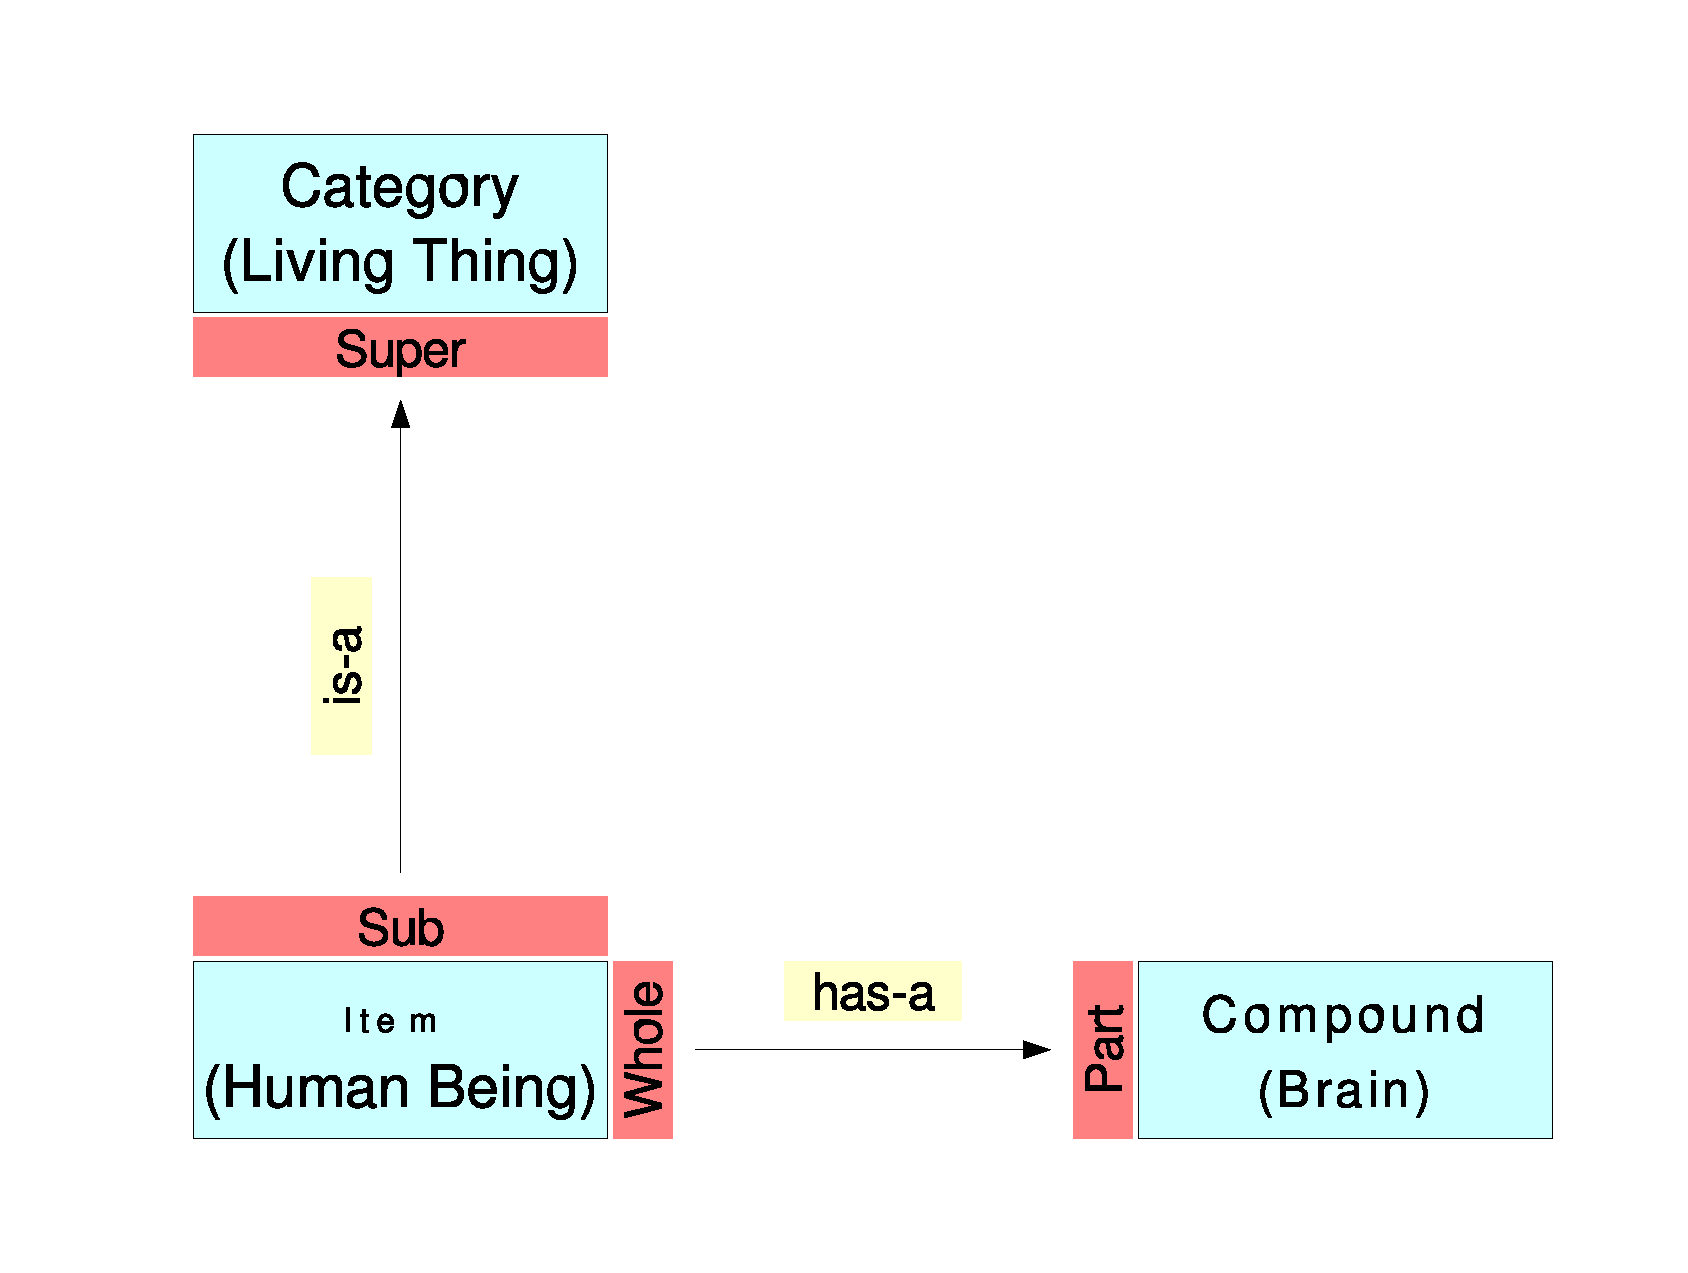
\includegraphics[width=10cm]{images/human_thinking.eps}
        \caption{Human Thinking}
        \label{human_thinking_figure}
      \end{center}
    \end{figure}
    
    \emph{Items} k�nnen �ber die "`has-a-Beziehung"' ein \emph{Compound} bilden und werden �ber die 
    "`is-a-Beziehung"' zu einer \emph{Category} zusammen gefasst. Wie sind diese Prinzipien in CYBOL umgesetzt?
    Jedes Template bzw. Laufzeitmodell vom Template repr�sentiert ein diskretes \emph{Item} bzw. 
    ein diskretes \emph{Compound}, was wiederum aus disketen \emph{Items} oder 
    \emph{Compounds} besteht. Die Abstraktion \emph{Category} ist in CYBOL nicht direkt als
    Beschreibung abgebildet, sondern muss
    �ber Operationen in CYBOL realisiert werden.
    
  \section{Architektur von CYBOP}
  
    CYBOP setzt sich aus verschieden Teilen zusammen. Dies beinhaltet einmal die Beschreibungssprache,
    dann einen Interpreter, der diese  Beschreibungssprache versteht und auf unterster Ebene 
    die Hardware, auf der die Operationen ausgef�hrt werden.
    
    \begin{itemize}
      \item Beschreibungssprache CYBOL \\
            Hier werden die Modelle beschrieben. Dazu geh�ren das Domain-Wissen, die Anwendungslogik
            und die Beschreibung der Oberfl�che f�r verschieden Ausgabemedien.
      \item Interpreter CYBOI \\
            Dies ist das Herzst�ck von CYBOP. Hier wird die Sprache CYBOL interpretiert. Dazu werden die Modelle
            gelesen, verarbeitet und f�r die verschiedenen Ausgabemedien die Anwendung generiert.
      \item Hardware \\
            Damit eine Anwendung funktioniert muss sie mit der Hardware zusammen arbeiten.  Dies muss durch den 
            CYBOP - Interpreter gew�hrleistet werden.
    \end{itemize}
    
    Die Beschreibungssprache CYBOL und der Interpreter CYBOI werden in den n�chsten Kapitel beschrieben. 
    Der Abschnitt Hardware ist f�r die Diplomarbeit nicht relevant.
    

  \chapter{Cybernetics Oriented Language (CYBOL)} 

  \section{�berblick}
    
    CYBOL ist die Beschreibungssprache von CYBOP f�r das Anwendungswissen, die
    Anwendungslogik und die Oberfl�chenbeschreibung. 
    CYBOL ist eine hierarchische Beschreibungssprache. Darum eignet sich f�r CYBOL
    das XML-Format, da XML genau f�r hierarchische Abbildungen gedacht ist.
    Dies hat den Vorteil, das vorhandene XML-Parser verwendet werden k�nnen.
    Weiterhin stehen XML-Editoren zur
    Erstellung und �berpr�fung der CYBOL-Dateien zur Verf�gung.
    In diesem Kapitel wird zuerst XML n�her erl�utert, danach wird CYBOL 
    in der XML-Syntax beschrieben und als letztes erfolgen
    die formellen Beschreibungen von CYBOL in DTD, XML-Schema und EBNF.

  \section{XML - Grundlage der Beschreibung von CYBOL}

    \subsection{Geschichtliches}
    
      Die Grundlage von CYBOL ist XML. XML ist ein Projekt der W3C und wird seit 
      Juli 1996 entwickelt. Urspr�nglich war XML als Alternative zur 
      Hypertext Markup Language (HTML), der Auszeichnungssprache f�r
      Internetseiten, gedacht. Es wurde jedoch schnell erkannt, das XML als 
      eine universelle Sprache zur Verwaltung und zum Austausch semantisch 
      qualifizierter Daten genutzt werden kann. Im November 1996 wurde 
      XML als Entwurf vorgestellt und hat seit Februar 
      1998 in der Version XML 1.0 den Status "`Empfehlung des W3C"'. XML stellt
      eine Teilmenge der Standard Generalized Markup Language (SGML) dar.

    \subsection{Definition von XML}
    
      Hier folgt nun eine kurze Erl�uterung, was XML eigentlich ist \cite[Seite 618]{defxml}.
      \begin{quotation}
        Der Inhalt eines XML-Dokuments besteht aus strukturierten Elementen,
        die hierarchisch geschachtelt sind. Dazwischen befindet sich der Inhalt,
        der aus weiteren Elementen (daher hierarchisch) und reinen Text bestehen kann.
        Die Elemente k�nnen Attribute enthalten, die zus�tzliche Informationen
        in einem Element ablegen.
      \end{quotation}
      Ein weiterer Begriff in Zusammenhang mit XML ist die Wohlgeformtheit eines Dokumentes. 
      Jedes XML-Dokument muss der Wohlgeformtheit gen�gen, das bedeutet dass jedes 
      XML-Dokument einer speziellen Spezifikationen entspricht.
      Diese Spezifikation ist im Detail hier aufgelistet:
      \begin{itemize}
        \item Jedes Element besteht aus einem Begin-Tag und einem End-Tag.
        \item Es gibt genau ein Wurzelelement, unter dem sich ein hierarchischer Baum aufbaut.
        \item Elemente m�ssen sauber ineinander eingebettet sein. Es darf 
              keine �berdeckungen geben.
        \item Alle Attributwerte m�ssen in Anf�hrungsstrichen stehen.
        \item Der Name eines Attributs kommt innerhalb eines Elements nicht mehr als einmal vor.
        \item Ein Attributwert darf keinen Verweis auf ein externes Entity enthalten.
      \end{itemize}
      
    \subsection{Syntax von XML}
    
      Die folgenden Ausf�hrungen beziehen sich auf die XML-Spezifikation des W3C \cite{w3c}.
      Dabei werden nur die Teile beschrieben, die auch in CYBOL verwendet werden. 

      \textbf{Struktur von XML-Dokumenten} \\
        Ein XML-Dokument besteht aus einem optionalen Prolog, einem Rumpf sowie aus einem
        optionalen Epilog. Ein Dokument kann wohlgeformt sein, ohne einen Prolog oder Epilog 
        zu haben. 
        
        Der Prolog kann die XML-Deklaration, die Informationen 
        �ber die verwendete XML-Spezifikation, die Zeichenkodierung, sowie die verwendeten 
        Entities enthalten. Hier ist ein Beispiel f�r einen Prolog, so wie er auch in 
        CYBOP verwendet wird, zu sehen:
        \begin{verbatim}
          <?xml version="1.0" encoding="iso-8859-1" standalone="yes"?>
        \end{verbatim}

        Der Rumpf ist der wichtigste Teil des XML-Dokumentes, da hier die eigentlichen
        Informationen abgelegt werden. Er besteht aus einem Element oder mehreren ineinander
        verschachtelten, Elementen.

        Der Epilog eines Dokumentes ist der Abschnitt nach dem Rumpf und steht f�r 
        Kommentare und Verarbeitungsanweisungen zur 
        Verf�gung. Die Verwendung dieses Abschnittes ist bisher nicht klar definiert, 
        deshalb ist eine sinnvolle Nutzung nur mit eigenen Applikationen m�glich.
        %Der Epilog wird in CYBOL nicht verwendet.
      
      \textbf{Elemente} \\
        Elemente sind die Grundbausteine eines XML-Dokumentes. Ein Element ist ein Container
        f�r beliebige Inhalte, wie zum Beispiel verschiedene Zeichen, weitere Elemente sowie andere
        Informationen. Begin-Tag und End-Tag begrenzen ein Element. Sie bestehen aus dem Namen
        des Elementyps, der in spitzen Klammern eingeschlossen wird. 
        \begin{verbatim}
          <Elementname> Elementinhalt </Elementname>
        \end{verbatim}
        Elemente ohne Inhalt werden als leere Elemente bezeichnet und k�nnen durch eine
        spezielle Schreibweise angegeben werden.
        \begin{verbatim}
          <Leerelement />
        \end{verbatim}
        Soll ein Dokument wohlgeformt sein, muss es eine baumartige Struktur aufweisen. In
        jedem Dokument darf es nur genau einen Baum geben, dessen Wurzel als \emph{document root}
        bezeichnet wird. Dieses Element ist das Elternelement aller anderen
        enthaltenen Elemente (Kinderelemente). Jede Wurzel eines Kinderelements muss 
        mindestens in einen Teilbaum enthalten sein, dessen Wurzel das \emph{document root} ist. 
        Die Verschachtelung der Elemente ist strikt
        einzuhalten, das hei�t ein Element muss seine Begin-Tags und End-Tags auf derselben
        Verschachtelungsebene haben.
      
      \textbf{Attribute} \\
        Attribute sind Teile von Elementen, die Informationen �ber deren Inhalt enthalten und
        nicht selbst zum Inhalt geh�ren. Attribute k�nnen in Begin-Tags von Elementen und
        Leerelementen angegeben werden und haben immer die Form:
        \begin{verbatim}
          Attributname="Attributwert"
        \end{verbatim}
        Die Attributwerte m�ssen immer Text-Literale sein. 
        Text-Literale sind ganz normale Zeichenketten, die von Begrenzungszeichen 
        (\verb|" oder '|) eingeschlossen
        werden. Dabei ist darauf zu achten, dass am Anfang und Ende dasselbe
        Begrenzungszeichen steht und das dieses nicht in der Zeichenkette
        verwendet wird.
      
      \textbf{Kommentare} \\
        S�mtliche Anmerkungen in Dokumenten, die nicht zum Inhalt geh�ren, werden als
        Kommentare gekennzeichnet. Die Syntax von XML f�r Kommentare ist
        \begin{verbatim}
          <!-- Hier steht ein Kommentar -->
        \end{verbatim}
        Diese erm�glichen es, Anmerkungen aufzunehmen,
        Entwicklungsschritte zu dokumentieren oder verschiedene andere Informationen
        einzuf�gen, die nur f�r den Leser des Quelltextes bestimmt sind.

      Weiter Informationen zu XML sind direkt auf den Seiten des W3C \cite{w3c} 
      bzw. in der deutschen �bersetzung \cite{w3cger} zu finden.

  \section{Beschreibung von CYBOL}
  
    Nachdem XML und ihre Syntax gekl�rt ist, kann die spezielle Syntax von CYBOL 
    dargelegt werden. 
    Ein wichtiger Aspekt
    von CYBOL ist die Einfachheit der Beschreibung. Darum werden alle Modelle
    nach dem gleichen Schema beschrieben, egal, ob es sich um die Anwendungslogik,
    die Oberfl�chenbeschreibung oder die Domainbeschreibung handelt. Diese CYBOL-Dateien
    werden auch Templates genannt, da aus diesen die Laufzeitmodelle in CYBOI 
    aufgebaut werden. 
    
    \subsection{Aufbau von CYBOL}   
      Eine CYBOL-Datei ist immer ein XML-Dokument. Es besteht aus dem Prolog und dem Rumpf. 
      Der Epilog wird in CYBOL nicht verwendet. Der Prolog
      setzt sich aus der XML-Deklaration und einer Beschreibung zusammen. 
      \begin{verbatim}
        <?xml version="1.0" encoding="iso-8859-1" standalone="yes"?>
        <!--
          Copyright and Description for the CYBOL file
        /-->
      \end{verbatim}
      Der Rumpf von CYBOL ist hierarchisch mit Elementen und den dazugeh�rigen Attributen 
      aufgebaut.
      Ein Rumpf sieht beispielhaft folgenderma�en aus:
      \begin{verbatim}
        <model>
          <part name="addresses" ...">
            <property name="whole" ..." >
              <constraint name="color" ... />
              ...
            </property>
            ...
          </part>
          ...
        </model>
      \end{verbatim}
      

    \subsection{Elemente von CYBOL}

      In dem Rumpf k�nnen bis zu vier Elementtypen verwendet werden. Diese Elementtypen
      sind hierarchisch aufgebaut.
      \begin{verbatim}
        model --> part --> property --> constraint
      \end{verbatim}
      Die Elementtypen haben folgende Bedeutung:
      \begin{table}[H]
        \centering
          \begin{tabular}{|l|p{10cm}|}
            \hline
            \textbf{Elementtyp} & \textbf{Beschreibung}
            \\ \hline
            model & 
            Dieses Element ist das Wurzelelement. Alle anderen Elemente sind ihm untergeordnet.
            \\ \hline
            part & 
            Jedes Modell besteht aus einem oder mehreren \emph{parts}. Dies kann zum Beispiel ein
            Datenelement sein oder auch eine Operation. Voneinander abh�ngige \emph{parts}
            werden hierarchisch aufgebaut (siehe dazu \ref{abbhierarchie}).
            \\ \hline
            property & 
            Beschreibt die Eigenschaften zu den \emph{parts}. Ein Beispiel w�re zu einer
            Sendeoperation die Eigenschaften des Senders und des Empf�ngers 
            zu definieren.
            \\ \hline
            constraint & 
            Unterliegen die \emph{properties} bestimmten Bedingungen, 
            die z.B. einen eingeschr�nkten Wertebereich 
            darstellen k�nnten, so werden diese hier definiert.
            \\ \hline
          \end{tabular}
        \caption{Elemente von CYBOL}
        \label{tab:ElementeVonCYBOL}
      \end{table}
      Andere Elementtypen sind in CYBOL nicht erlaubt. 
      Die Elementtypen \emph{property} und \emph{constraint} m�ssen
      nicht immer angegeben werden, sondern nur, wenn es im Kontext zu den Elementtyp \emph{part} sinnvoll ist. 

    \subsection{Attribute der Elemente von CYBOL}
      F�r die vollst�ndige Beschreibung wird nun auf die Attribute der Elemente eingegangen.
      Auch hier gibt es immer die gleichen Attribute, egal um welche Beschreibung es sich handelt.
      Die Attribute in den Elementen haben folgende Bedeutung:
      
      \begin{table}[H]
        \centering
          \begin{tabular}{|l|p{10cm}|}
            \hline
            \textbf{Attribut} & \textbf{Beschreibung}
            \\ \hline
            name & 
            Das Attribut \emph{name} ist die Bezeichnung f�r den Eintrag. In Abh�ngigkeit 
            von dem zu beschreibenden Element ist dieser frei w�hlbar (bei Element part) 
            oder durch den Kontext
            bestimmt. Ein Beispiel f�r einen Name mit einer bestimmten Bedeutung w�re 
            f�r das Element \emph{property} der Name \emph{color} f�r die Farbe des \emph{part}.
            \\ \hline
            channel & 
            Dieses Attribut beschreibt, wie der Eintrag im Attribut \emph{model} zu lesen ist.
            Dies k�nnte \emph{inline} sein,
            wenn die Beschreibung im Attribut \emph{model} enthalten ist oder es 
            k�nnte \emph{file}
            annehmen, wenn im  Attribut \emph{model} auf eine weitere CYBOL-Datei 
            verwiesen wird.
            \\ \hline
            abstraction & 
            Dies entspricht im herk�mmlichen Sinne dem Datentyp. Bei einfachen Datentypen w�re dies 
            \emph{string}, \emph{integer}, \emph{float} oder \emph{vector}. Bei zusammengesetzten 
            Datentypen w�rde dies \emph{cybol} entsprechen. F�r eine primitive
            Operation der Anwendungslogik w�rde der Wert \emph{operation} hei�en.  
            \\ \hline
            model & 
            Dies ist abh�ngig von der \emph{abstraction}. Bei einfachen Datentypen kann im 
            Attribut \emph{model} ein Wert zugewiesen werden.
            Bei Operationen wird hier die auszuf�hrende Operation definiert. Ist die \emph{abstraction}
            gleich \emph{cybol}, so wird im \emph{model} auf eine weitere CYBOL-Datei verwiesen.
            \\ \hline
          \end{tabular}
        \caption{Attribute der Elemente von CYBOL}
        \label{tab:AttributeDerElementeVonCYBOL}
      \end{table}
      Dies ist die allgemeine Beschreibung von CYBOL. Was jetzt noch fehlt, ist die Definition,
      welche Werte die einzelnen Attribute der Elemente annehmen k�nnen und in welcher Kombination
      sie sinnvoll sind. CYBOL ist noch in der Anfangsphase der Entwicklung und wird
      systematisch weiter ausgestaltet. Bei  der Beispielanwendung, die im Rahmen der Diplomarbeit entsteht, 
      werden diese Werte f�r die einzelnen Attribute der Elemente beschrieben.
      
    \subsection{Abbildung von Hierarchien}
      \label{abbhierarchie}
      Nicht nur der Aufbau der Beschreibungssprache ist hierarchisch, sondern auch die Abbildungen
      der \emph{part}. Ein Teil setzt sich aus mehreren Teilen zusammen. Dies wird in 
      CYBOL �ber mehrere Dateien gel�st. 
      Innerhalb des Elements part kann keine Hierarchie abgebildet werden, sondern dies geschieht �ber 
      die Einbindung weiterer CYBOL-Dateien mit den  Attributen     
      \verb|channel="file"|, \verb|abstraction="cybol"| und 
      \verb|model="?model?"|, wobei \verb|?model?| f�r das entsprechende hierarchisch 
      untergeordnete CYBOL-Modell steht.
      Ein kleines Beispiel k�nnte so aussehen:
      \begin{verbatim}
        <model>
          <part name="table" channel="file" 
                abstraction="cybol" model="part_of_table.cybol" />
        </model>
      \end{verbatim}
      Hier wird der \emph{part} Tisch definiert. In der Datei part\_of\_table.cybol sind die parts Tischplatte
      und die 4 Tischbeine definiert.
      \begin{verbatim}
        <model>
          <part name="tabletop" channel="inline" 
                abstraction="vector" model="50,50,5" />
          <part name="tableleg1" channel="inline" 
                abstraction="vector" model="5,5,30" />
          ...
        </model>
      \end{verbatim}
      
  \section{Formelle Beschreibungen von CYBOL}
      
    F�r die formelle Beschreibung von CYBOL gibt es verschiedene M�glichkeiten. Da
    CYBOL in XML beschrieben wird, sind die Meta-Beschreibungen von XML als formelle
    Beschreibung m�glich. Dies beinhaltet die  Document Type Definition, kurz DTD, und
    die XML-Schemata. Eine weitere M�glichkeit f�r die formelle Beschreibung besteht in der 
    Backus-Naur-Form (BNF) bzw. in der erweiterten Backus-Naur-Form (EBNF). 
    
    \subsection{Document Type Definition (DTD)}

      Eine Document Type Definition, kurz DTD, beschreibt den strukturellen Aufbau und die
      logischen Elemente einer Klasse von Dokumenten, genannt Dokumententyp. Die DTD ist
      eine Mustervorlage f�r eine Sammlung gleichartiger Dokumente. Ein Editor kann dieses
      Muster schon beim Schreiben mit dem aktuellen Dokument vergleichen und auf
      strukturelle Fehler, z.B. fehlende Elemente, hinweisen. Ohne DTD kann kein Programm
      entscheiden, welche Elemente zu einem Dokument geh�ren und ob sie zwingend
      notwendig sind.
      
      Die Angabe der DTD erfolgt in einem XML-Dokument mit der DOCTYPE-Deklaration. Dabei
      wird zwischen interner und externer Deklaration unterschieden. Bei einer internen
      Deklaration wird die DTD innerhalb der DOCTYPE-Deklaration angegeben, bei der
      externen Deklaration wird auf eine separate DTD verwiesen. CYBOL verwendet
      die DOCTYPE-Deklaration f�r die DTD nicht. Darum brauchen sie in CYBOL-Dateien 
      weder intern noch extern referenziert werden.

      \textbf{Elemente}\\
      Elemente sind das Kernst�ck von XML-Dokumenten. Sie werden in der DTD durch das
      Tag \verb|<!ELEMENT name (wert) >| definiert. Dabei steht 'name' f�r den Namen des 
      Elements und f�r 'wert' k�nnen die Werte 'EMPTY', 'ANY', 'PCDATA' (als Datentyp)
      oder weitere untergeordnete Elemente eingetragen sein. Bei untergeordneten 
      Elementen kann noch unterschieden werden, wie oft diese Elemente
      vorkommen d�rfen (? einmal oder gar nicht, * keinmal, einmal oder beliebig oft, 
      + mindestens einmal). Weiterhin besteht die M�glichkeit, 
      Sequenzen von Elementen ( ',' zwischen den
      Elementen) oder Alternativen von Elementen ('|' zwischen den Elementen) zu definieren.
      
      \textbf{Attribute} \\
      Attribute bieten die M�glichkeit, Elemente zu erweitern und zu modifizieren. Mit ihrer
      Hilfe k�nnen zum Element geh�rende Informationen angegeben werden. Diese Attribute
      werden auch innerhalb der DTD definiert. Alle Elemente, denen Attribute zugeordnet sind,
      erhalten in der DTD eine Attributliste mit dem Tag 
      \verb|<!ATTLIST name typ vorgabewert >|. Jede
      Attributdefinition besteht aus einem Namen, dem Typ und einem optionalen Vorgabewert.
      Typ ist im einfachsten Fall CDATA, f�r Vorgabewerte k�nnen z.B. \#REQUIRED (erforderlich)
      oder \#IMPLIED (optional) eingetragen werden.

      \textbf{DTD f�r CYBOL}\\
      Hier folgt nur die komplette DTD f�r CYBOL. Da sie nicht in den CYBOL-Dateien referenziert wird,
      ist dies nur eine formale Beschreibung von CYBOL.
      \begin{verbatim}
        <!ELEMENT model (part*)>
        <!ELEMENT part (property*)>
        <!ELEMENT property (constraint*)>
        <!ELEMENT constraint EMPTY>
        
        <!ATTLIST part
            name CDATA #REQUIRED
            channel CDATA #REQUIRED
            abstraction CDATA #REQUIRED
            model CDATA #REQUIRED>
        
        <!ATTLIST property
            name CDATA #REQUIRED
            channel CDATA #REQUIRED
            abstraction CDATA #REQUIRED
            model CDATA #REQUIRED>
        
        <!ATTLIST constraint
            name CDATA #REQUIRED
            channel CDATA #REQUIRED
            abstraction CDATA #REQUIRED
            model CDATA #REQUIRED>
      \end{verbatim}
      

    \subsection{XML - Schema}
      
      XML-Schema ist ein neuer Ansatz zur Definition von Dokumententypen. Mit der
      Entwicklung von XML hatte sich zun�chst die von der SGML �bernommene DTD als
      Format zur Beschreibung konkreter Dokumententypen etabliert. Mit der zunehmenden
      Verbreitung von XML in der Praxis machten sich zunehmend die Grenzen und Nachteile
      der DTD bemerkbar. Besonders die dokumentenzentrierte Sichtweise der DTD unter
      Vernachl�ssigung von Datentypen erwies sich als Problem. So lie�en
      DTD weder die Beschreibung bestimmter semantischer Bedingungen noch die Festlegung
      von Wertebereichen zu. Gerade die zunehmende Verbreitung verteilter Anwendungen
      erfordert es, Daten in einem einheitlichen, aber flexiblen und leicht modifizierbaren
      Format, das sich einfach parsen l�sst, zu transportieren. F�r die L�sung des Problems sollte
      eine XML-basierte Sprache genutzt werden. Daraus entstand das XML-Schema.
      
      Die komplette Beschreibung von XML - Schema w�rde den Rahmen dieser Arbeit sprengen. 
      Darum wird nur auf die Elemente eingegangen, die in der Beschreibung f�r CYBOL notwendig sind. 
      Weitere Informationen zu XML-Schemata sind unter \cite{xsd} zu finden. 
      \textbf{Namensraum} \\
        Im Wurzelelement des Schemas wird der aktuelle Namensraum f�r Schemata nach W3C
        Version 1.0, bezogen auf die dort definierten Strukturen, angegeben:
        \begin{verbatim}
          xmlns:xs="http://www.w3.org/2001/XMLSchema"
        \end{verbatim}
        Der Namensraum wird nun durch den Alias \verb|xs| repr�sentiert.
        Der definierte Alias wird im Dokument dann vor allen Elementen, Attributen und
        Datentypen mit angegeben, so das die Beschreibung innerhalb des Namensraums eindeutig ist.
      
      \textbf{Komplexe Elementtypen} \\
        Das Element complexType dient zur Definition eines Elementtyps, welcher weitere
        Unterelemente beinhalten kann. Das Attribut name definiert den Bezeichner dieses
        Elementtyps. Die Reihenfolge und Auswahl der Unterelemente kann durch folgende Kompositoren
        angegeben werden:  
        \begin{table}[H]
          \centering
            \begin{tabular}{|l|l|} 
              \hline
              \textbf{Kompositor} & \textbf{Bedeutung} \\ \hline
              sequence & Vorgegebene Reihenfolge de Subelemente \\ \hline
              choice & Auswahl eines der Subelemente \\ \hline
              all & Alle Subelemente oder keines, Reihenfolge ist egal \\ \hline
            \end{tabular}
          \caption{Kompositoren komplexer Elemente}
          \label{tab:KompositorenKomplexerElemente}
        \end{table}
        
      \textbf{Elemente} \\
        Zur Deklaration eines Elementes in einem XML-Schema reichen die Angabe eines Namens und
        eines Typs als Attribute des Elementes <element>. Durch die Attribute minOccurs 
        und maxOccurs kann zus�tzlich angegeben werden,
        wie oft das Element mindestens bzw. maximal hintereinander auftreten darf.
        \begin{verbatim}
          <xs:element name="MyElement" type="xs:string"/>
        \end{verbatim}
        
      \textbf{Attribute} \\
        Attributdeklarationen erscheinen am Schluss einer Elementbeschreibung. Ihre Angabe
        erfolgt durch das Element <attribute>, das die Attribute name und type hat. 
        Mit dem Attribut use kann angeben werden, ob das entsprechende Attribut definiert werden muss.
        Folgende Deklaration beschreibt ein Attribut:
        \begin{verbatim}
          <xs:attribute name="MyAttribute" type="xs:string"/>
        \end{verbatim}
      
      
      \textbf{XML-Schema f�r CYBOL} \\
      Hier folgt nun das komplette XML-Schema f�r CYBOL. Da dieses Schema, wie auch die DTD nicht
      in den CYBOL-Dateien referenziert wird, ist dies auch nur eine formelle Beschreibung von CYBOL.
      
      \begin{verbatim}
<xs:schema 
  xmlns:xs='http://www.w3.org/2001/XMLSchema'
  targetNamespace='http://www.cybop.net'
  xmlns='http://www.cybop.net'
  elementFormDefault='qualified'>
  <xs:element name='model'>
    <xs:complexType>
      <xs:sequence>
         <xs:element ref='part' minOccurs='0' maxOccurs='unbounded'/>
      </xs:sequence>
    </xs:complexType>
  </xs:element>
  <xs:element name='part'>
    <xs:complexType>
      <xs:sequence>
        <xs:element ref='property' minOccurs='0' maxOccurs='unbounded'/>
      </xs:sequence>
      <xs:attribute name='name' type='xs:string' use='required'/>
      <xs:attribute name='channel' type='xs:string' use='required'/>
      <xs:attribute name='abstraction' type='xs:string' use='required'/>
      <xs:attribute name='model' type='xs:string' use='required'/>
    </xs:complexType>
  </xs:element>
  <xs:element name='property'>
    <xs:complexType>
      <xs:sequence>
        <xs:element ref='constraint' minOccurs='0' maxOccurs='unbounded'/>
      </xs:sequence>
      <xs:attribute name='name' type='xs:string' use='required'/>
      <xs:attribute name='channel' type='xs:string' use='required'/>
      <xs:attribute name='abstraction' type='xs:string' use='required'/>
      <xs:attribute name='model' type='xs:string' use='required'/>
    </xs:complexType>
  </xs:element>
  <xs:element name='constraint'>
    <xs:complexType>
      <xs:attribute name='name' type='xs:string' use='required'/>
      <xs:attribute name='channel' type='xs:string' use='required'/>
      <xs:attribute name='abstraction' type='xs:string' use='required'/>
      <xs:attribute name='model' type='xs:string' use='required'/>
    </xs:complexType>
  </xs:element>
</xs:schema>      
      \end{verbatim}
      
    \subsection{Erweiterte Backus-Naur-Form (EBNF)}
    
      Die Grammatik einer formalen Sprache regelt die Rechtschreibung. Sie legt die korrekte 
      Syntax fest. Es gibt unterschiedliche Notationen f�r Grammatiken. Eine 
      einfache und ausdrucksstarke Form ist die Erweiterte 
      Backus-Naur-Form (EBNF). Seltener verwendet wird die urspr�ngliche, 
      einfache Backus-Naur-Form (BNF). Dieser fehlen gegen�ber der EBNF ein paar 
      bequeme, abk�rzende Schreibweisen. Mit beiden Formen lassen sich aber dieselben 
      Grammatiken wiedergeben.
      
      Mit EBNF lassen sich Grammatiken vom Typ 2 der Chomsky-Hierarchie darstellen.
      Dies sind kontextfreie Grammatiken, das bedeutet das die Grammatik 
      $G=\left( N, \Sigma, P, S \right)$ mit N gleich Menge der Nichtterminalsymbole,
      $\Sigma$ gleich Menge der Terminalsymbole, P gleich die Menge von Regeln und 
      S gleich das Startsymbol, folgenden Einschr�nkungen unterliegen:
      \begin{displaymath}      
        \forall ( w_1 \rightarrow w_2 ) \in P : \left| w_1 \right| \le \left| w_2 \right|
      \end{displaymath}
      \begin{displaymath}      
        \forall ( w_1 \rightarrow w_2 ) \in P : w_1 \in N
      \end{displaymath}
      CYBOL ist eine kontextfreie Grammatik und kann somit in der EBNF
      notiert werden. 

      Mit EBNF lassen sich auch Grammatiken vom Typ 3 der Chomsky-Hierachie darstellen.
      Dazu m�ssen zus�tzlich
      die folgenden Bedingungen eingehalten werden:
      \begin{displaymath} 
        \forall (w_1 \rightarrow w_2) \in P : w_1 \in N 
      \end{displaymath} 
      \begin{displaymath} 
        w_2 \in \Sigma \cup \Sigma \cdot N \cup \{ \epsilon \}
      \end{displaymath} 
      
      Schon die erste Regel in der EBNF von CYBOL widerspricht der zus�tzlichen Regel.
      \begin{verbatim}
        CYBOL   = '<model>' 
                    {part}
                  '</model>';
      \end{verbatim}
      Auf der rechten Seite der Regel d�rfen nur Terminalsymbole oder Terminalsymbole gefolgt von einem
      Nichtterminalsymbol stehen. Somit entspricht CYBOL keine Grammatik vom Typ 3 der 
      Chomsky-Hierarchie.
      
      \textbf{Syntax von EBNF} \\

        Die folgende �bersicht gibt die verwendeten Beschreibungskonstrukte von EBNF \cite{ebnf}
        wieder:
        \begin{table}[H]
          \centering
            \begin{tabular}{|l|l|} 
              \hline
              \textbf{Zeichen} & \textbf{Bedeutung} \\ \hline
              = & Definition \\ \hline
              ; & Endezeichen \\ \hline
              | & Logisches Oder \\ \hline
              [...]  & Option \\ \hline
              {...}  & Optionale Wiederholung \\ \hline
              (...)  & Gruppierung \\ \hline
              "..."  & Anf�hrungszeichen, 1. Variante \\ \hline
              '...'  & Anf�hrungszeichen, 2. Variante \\ \hline
              (*...*)  & Kommentar \\ \hline
            \end{tabular}
          \caption{Syntax von EBNF}
          \label{tab:SyntaxVonEBNF}
        \end{table}
      
      \textbf{EBNF f�r CYBOL} \\
      Hier folgt die vollst�ndige Notation von CYBOL in der EBNF. 
\begin{verbatim}
CYBOL   = '<model>' 
              {part}
          '</model>';
          
part    = '<part ' all_attribute '\>' |
          '<part ' all_attribute '>'
              {property}
          '</part>';

property    = '<property ' all_attribute '\>' |
              '<property ' all_attribute '>'
                  {constraint}
              '</property>';

constraint  = '<constraint ' all_attribute '\>';

all_attribute          = attribute_name attribute_channel 
                         attribute_abstraction attribute_model

attribute_name          = 'name="' name '"';
attribute_channel       = 'channel="' channel '"';
attribute_abstraction   = 'abstraction="' abstraction '"';
attribute_model         = 'model="' model '"';

name            = description_sign;
channel         = description_sign;
abstraction     = description_sign;
model           = value_sign;

description_sign    = { ( letter | number ) } ;
value_sign          = { ( letter | number | other_sign ) } ;

letter          = small_letter | big_letter;
small_letter    = 'a' | 'b' | 'c' | 'd' | 'e' | 'f' | 'g' |
                  'h' | 'i' | 'j' | 'k' | 'l' | 'm' | 'n' |
                  'o' | 'p' | 'q' | 'r' | 's' | 't' | 'u' |
                  'v' | 'w' | 'x' | 'y' | 'z';
big_letter      = 'A' | 'B' | 'C' | 'D' | 'E' | 'F' | 'G' |
                  'H' | 'I' | 'J' | 'K' | 'L' | 'M' | 'N' |
                  'O' | 'P' | 'Q' | 'R' | 'S' | 'T' | 'U' |
                  'V' | 'W' | 'X' | 'Y' | 'Z';     
other_sign      = ',' | '.' | '/', '+', '-', '*';                  
number          = '0' | '1' | '2' | '3' | '4' | 
                  '5' | '6' | '7' | '8' | '9';   

\end{verbatim}
      
      

  \section{Logik von CYBOL}
  
    Mit der Beschreibungssprache CYBOL wird das statische und dynamische Verhalten 
    einer Anwendung dargestellt. Dazu bedarf es der folgenden Grundkonstrukte, um 
    das Wissen und die Logik einer Anwendung zu beschreiben.
    \begin{enumerate}
      \item Sequential
      \item Selection
      \item Iteration
    \end{enumerate}
    In den weiteren Abschnitten wird die Darstellung dieser Konstrukte 
    f�r CYBOL beschrieben.
    
    \subsection{Sequential}
      
      Die Ausf�hrung von mehreren Befehlen hintereinander wird 
      als sequentielle Abarbeitung bezeichnet. Im ersten Schritt 
      wird dies durch die 
      Reihenfolge in den CYBOL-Beschreibungsdateien bestimmt.
      In Zukunft k�nnte auch die Reihenfolge �ber ein Property \emph{position}
      innerhalb der CYBOL-Datei gesteuert werden. 
      Dies h�tte den Vorteil, dass unabh�ngig von der Position innerhalb 
      der CYBOL-Datei die Abarbeitungsreihenfolge festgelegt werden kann. F�r
      diese Flexibilit�t w�rde aber die CYBOL-Datei un�bersichtlicher,
      da die Reihenfolge der Abarbeitung nicht der Reihenfolge der 
      Position in der CYBOL-Datei entsprechend w�rde.

    \subsection{Selection}
    
      Eine weitere wichtige Funktion zur Ablaufsteuerung ist die \emph{selection}. Dies 
      erm�glicht Verzweigungen innerhalb der Programmausf�hrung. Daf�r gibt es in CYBOL
      die Operation \emph{selection} mit den Properties \emph{comparison}, 
      \emph{true\_model} und \emph{false\_model}. Die Eigenschaft \emph{comparison} 
      ist vom Typ Boolean und dient als Vergleichs-Flag zur Unterscheidung, welches Modell 
      ausgef�hrt werden soll. Eine Verzweigung wird in CYBOL folgenderma�en definiert:
\begin{verbatim}      
<part name="selection" channel="inline" 
      abstraction="operation" model="selection">
    <property name="comparison" channel="inline" 
              abstraction="knowledge" model="domain.comparisonflag"/>
    <property name="true_model" channel="file" 
              abstraction="cybol" model="true_model.cybol"/>
    <property name="false_model" channel="file" 
              abstraction="cybol" model="false_model.cybol"/>
</part>
\end{verbatim}      
    

    \subsection{Iteration}
    
      Iteration ist eine Schleifenkonstrukt. In der prozeduralen  
      Programmierung gibt es bis zu drei verschiedene Schleifentypen, die \emph{repeat until},
      die \emph{for} und die \emph{while do} Schleife. Diese Schleifentypen sind alle 
      ineinander umwandelbar. Darum gibt es in CYBOL nur eine Iterationsform. 
      Diese ist folgenderma�en definiert.
      
\begin{verbatim}      
<part name="creat_table_body" channel="inline" 
      abstraction="operation" model="loop">
    <property name="break" channel="inline" 
              abstraction="knowledge" model="domain.loop_breakflag"/>
    <property name="index" channel="inline" 
              abstraction="knowledge" model="domain.loop_index"/>
    <property name="model" channel="file" 
              abstraction="cybol" model="create_table_rows.cybol"/>
</part>
\end{verbatim}      
      \newpage
      Es gibt eine Operation \emph{loop}, die die Eigenschaften \emph{break}, \emph{index}
      und \emph{model} hat. 
      Das \emph{model} wird solange ausgef�hrt,
      bis die Eigenschaft \emph{break} wahr ist. Das Modell f�r \emph{break} 
      ist vorher anzulegen, damit die Schleifenoperation das Breakflag auch auswerten kann.
      Weiterhin muss, soll keine Endlosschleife entstehen,  
      in dem \emph{model} die Eigenschaft \emph{break} manipuliert werden, so dass die Schleife
      eine Chance hat, sich zu beenden. In der Eigenschaft \emph{index}
      wird eine Z�hlvariable mitgez�hlt.
 

  \chapter{Cybernetics Oriented Interpreter (CYBOI)} 

  F�r die Beschreibungssprache CYBOL   ist zur Ausf�hrung ein
  Interpreter, genannt CYBOI, notwendig. Dieser Interpreter hat die Aufgabe, die CYBOL-Dateien zu 
  lesen, zu parsen und zu verarbeiten. Der Interpreter ist in C geschrieben.   
  In diesen Abschnitt wird der Interpreter vorgestellt, seine Arbeitsweise 
  beschrieben und die verwendeten Software- und Architektur-Pattern erl�utert.

  \section{Pattern in CYBOI}

    Sehr oft wiederholen sich die Probleme. Auch
    die L�sungsans�tze f�r diese sind identisch.
    Alles spricht daf�r, solche L�sungswege abstrakt zu beschreiben und
    zu benennen.   
    Ein Pattern umfasst die beteiligten Komponenten, 
    ihre Verantwortlichkeiten und Verbindungen. Die Pattern helfen somit auf 
    vorhandenes Expertenwissen zur�ckzugreifen. 

    Christoper Alexander definierte Pattern folgenderma�en \cite{defpattern}:
    \begin{quotation}
      Jedes Muster beschreibt ein in unserer Umwelt best�ndig wiederkehrendes Problem 
      und erl�utert den Kern der L�sung f�r dieses Problem, so dass man diese L�sung 
      beliebig oft anwenden kann, ohne sie jemals ein zweites Mal gleich auszuf�hren.
    \end{quotation}
    In den n�chsten Abschnitten werden einige Pattern, die in CYBOI verwendet werden,
    beschrieben. 

    \section{Pipes and Filters}
    
      Ein wichtiges Pattern in CYBOI ist \emph{Pipes and Filters} \cite{patternbuschmann}.
      \begin{quotation}
        Das Pipes-and-Filters-Muster bietet eine Struktur f�r Systeme, die Datenstr�me verarbeiten. 
        Jeder Verarbeitungsschritt ist dabei in einen Filter gekapselt. Daten werden durch 
        Kan�le (engl. pipe) von Filter zu Filter weitergegeben. Die Filter k�nnen immer wieder
        neu angeordnet werden, was es erm�glicht, eine Familie von verwandten Systemen zu erstellen. 
      \end{quotation}
      
      Das \emph{Pipes and Filters} Muster wird also verwendet, wenn die Ausgabe von einem Filter
      gleich f�r die Eingabe des n�chsten Filters verwendet wird. In dem Filter werden 
      die Transformationen des Datenstromes durchgef�hrt.
      
      Im CYBOI wird dieses Pattern bei der Behandlung (Erzeugen und Zerst�ren) von 
      CYBOI-Modellen verwendet. Dabei ist in CYBOI 
      die Unterscheidung von \emph{primitive model} und \emph{compound model} zu machen. 
      \emph{Primitive model} sind alle Modelle, die auf elementare Strukturen aufbauen.
      Dies beinhaltet alle primitiven Datentypen (Integer, Vector, ...), die in CYBOI implementiert sind
      und alle elementaren Operationen. \emph{Compound model} sind dagegen alle Modelle, die sich aus 
      weiteren Modellen zusammensetzen. 
      
      In den Abbildungen \ref{fig:pipesandfilters_1} und \ref{fig:pipesandfilters_2} sind die 
      in CYBOI verwendeten \emph{Pipes and Filters} zu sehen. Diese werden genutzt, um Modelle, die persistent
      vorliegen, in das System von CYBOI zu integrieren bzw. wieder persistent abzuspeichern. 

      \begin{figure}[H]
        \centering
          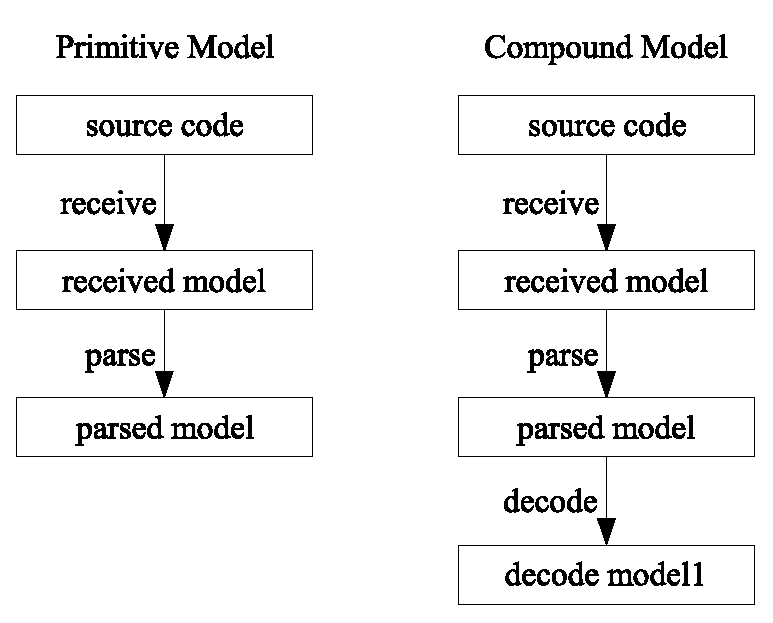
\includegraphics[width=9.5cm]{images/pipesandfilters_1.eps}
        \caption{decode model}
        \label{fig:pipesandfilters_1}
      \end{figure}
      \begin{figure}[H]
        \centering
          \includegraphics[width=9.5cm]{images/pipesandfilters_2.eps}
        \caption{encode model}
        \label{fig:pipesandfilters_2}
      \end{figure}

      Der \emph{source code}, der in einen persistenten Zustand vorliegt, wird geladen. Das 
      Ergebnis wird einen Parser
      �bergeben. Ist es ein \emph{primitive model}, so ist das geparste Ergebnis unser Modell.
      Bei einen \emph{compound model} wird das Ergebnis des Filters \emph{parse} noch decodiert,
      damit das Modell  hierarchisch aufgebaut wird. Diese Modelle liegen in einen 
      transienten Zustand vor. F�r die Abspeicherung von Modellen ist der umgekehrte Weg 
      n�tig. 
      
    \section{Compositum}
      
      Das Compositum Muster dient zur Darstellung von Teil-Ganzes-Hierarchien. 
      In CYBOI wird das gesamte Wissen in einer Baumstruktur gespeichert.
      Diese Baumstruktur setzt sich aus primitiven Typen und aus einer Container-Struktur,
      in CYBOI \emph{compound} genannt, zusammen. Diese Container-Struktur kann
      entweder primitive Typen oder weitere Container-Strukturen enthalten. Die untersten Bl�tter
      in der Baumstruktur sind immer primitive Typen. 
      
      \begin{figure}[H]
        \centering
          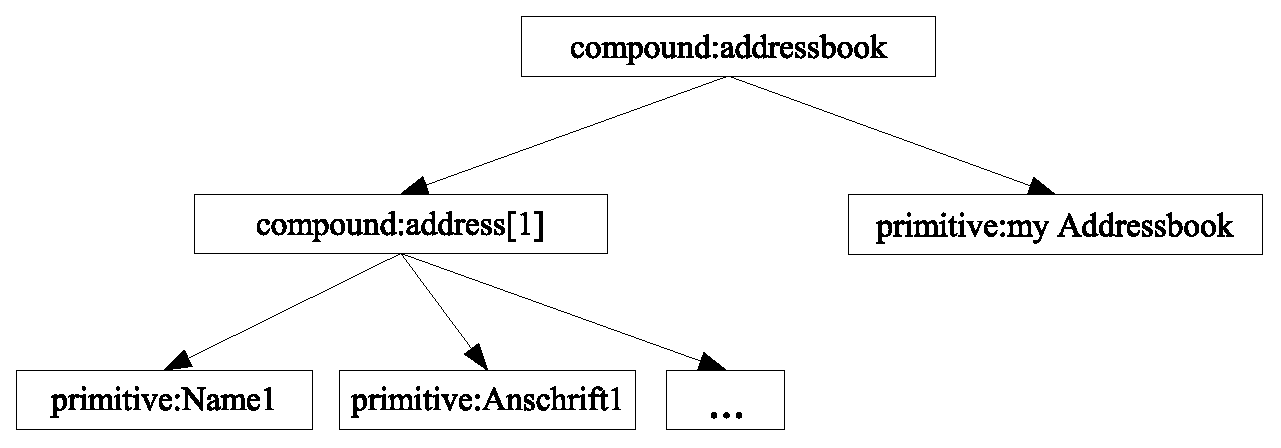
\includegraphics[width=15cm]{images/compositum.eps}
        \caption{Adressbuch als Compositum}
        \label{fig:compositum}
      \end{figure}

      Nach \cite{gamma04} wird dieses Muster verwendet, wenn keine Unterscheidung zwischen den Operationen
      von primitiven und zusammengesetzten Objekten gemacht werden soll. Da
      dieses Muster aus der objektorientierten Programmierung kommt, ist dies in CYBOI nur 
      partiell nutzbar. Das Prinzip des Patterns ist, bei der Ausf�hrung einer Operation 
      auf einer Komponente, diese Operation hierarchisch nach unten durchzureichen. 
      Da in CYBOI keine direkte Verkn�pfung von Operation und Daten vorliegt, ist
      dieser Teil des Patterns auch nicht nutzbar. Das Compositum Muster wird in CYBOI
      nur f�r die Abbildung der Beziehungen der einzelnen Komponenten verwendet,
      das aber konsequent f�r alle Daten, f�r alle Operation usw. 
      
  \section{Architektur von CYBOI}
  
    CYBOI beschr�nkt sich in seiner Architektur im Wesentlichen auf folgende zwei Container.
    \begin{itemize}
      \item Signal Memory
      \item Knowledge Memory
    \end{itemize}
    
    \subsection{Signal Memory} 
      Der \emph{Signal Memory} beschreibt die dynamische Komponente. Unter einen Signal versteht man die 
      Anweisung f�r die Ausf�hrung eines Befehles in CYBOI. 
      \emph{Signal Memory} ist eine Liste von allen noch abzuarbeitenden Signalen.
      In einer Endlosschleife werden diese Signale ausgef�hrt.  
      Nach der Abarbeitung werden die einzelnen Signale aus dem \emph{Signal Memory}
      entfernt. Die Reihenfolge der Abarbeitung von Signalen kann �ber Priorit�ten gesteuert werden.
      Ein Signal setzt sich aus den Bestandteilen, wie in Tabelle 
      \ref{tab:BestandteileEinesSignals} aufgelistet, zusammen.
      
      \begin{table}[H]
        \centering
          \begin{tabular}{|l|p{10cm}|}
            \hline
            \textbf{Bestandteil} & \textbf{Beschreibung }
            \\ \hline
            abstraction & 
            Dies beschreibt, in welcher Abstraktion das Modell vorliegt. Die 
            Abstraktion bestimmt somit, wie das Modell in CYBOI verarbeitet wird.
            \\ \hline
            model & 
            Dies ist das eigentliche Signal.
            \\ \hline
            detail & 
            Manche Signale brauchen f�r eine erfolgreiche Abarbeitung noch weitere 
            Parameter.
            \\ \hline
            priority & 
            �ber die Priorit�t kann die Reihenfolge der Signalabarbeitung beeinflusst werden.
            \\ \hline
            main signal id &
            Das Erzeugersignal bekommt eine eindeutige ID innerhalb von CYBOI. Erzeugt dieser
            Prozess weitere Signale, so wird auf den Erzeugerprozess verwiesen.
            \\ \hline
          \end{tabular}
        \caption{Bestandteile eines Signals}
        \label{tab:BestandteileEinesSignals}
      \end{table}

  
    \subsection{Knowledge Memory} 
      Der zweite Container \emph{Knowledge Memory} dient zur Speicherung unseres Wissens. Diesen Container 
      kann man sich als Baumstruktur vorstellen, in dem unser ganzes Wissen enthalten ist. 
      \emph{Knowledge Memory} enth�lt das aktuelle Wissen, das CYBOI zur Verf�gung steht.
      Eine Auswahl des Wissens ist in 
      Abbildung \ref{fig:knowledgememory} zu betrachten. Jedes Wissen wird in dieser
      Struktur gespeichert.
      \begin{figure}[H]
        \centering
          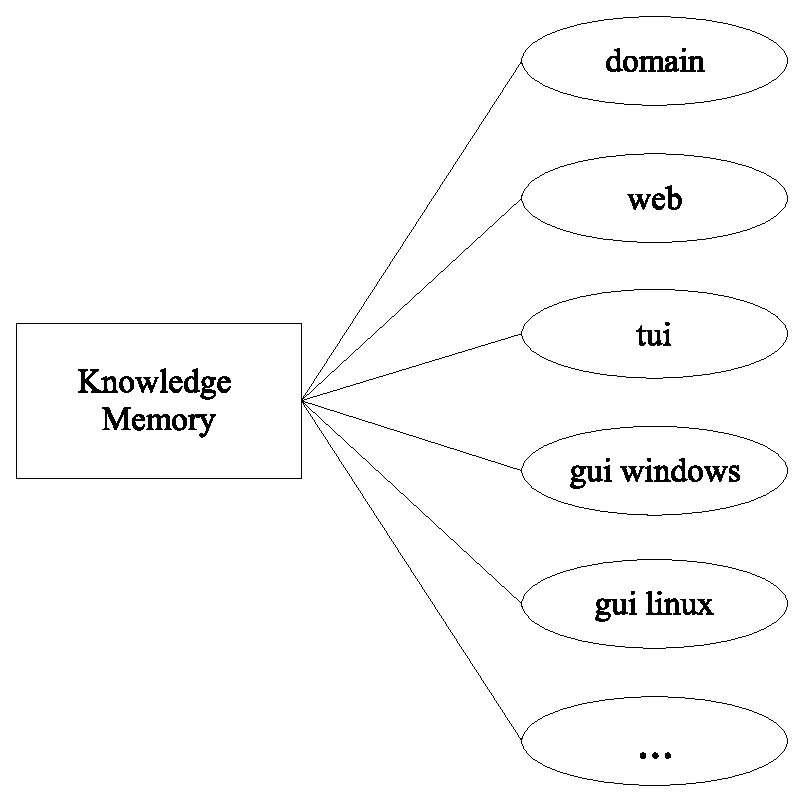
\includegraphics[width=8cm]{images/knowledgememory.eps}
        \caption{Knowledge Memory}
        \label{fig:knowledgememory}
      \end{figure}
    
    

    
  \section{Lifecycle von CYBOI}
  
    Das Grundger�st von CYBOI ist eine einfache Endlosschleife. In dieser Schleife wird immer wieder gepr�ft, 
    ob ein Signal f�r die Bearbeitung ansteht. Ist dies der Fall, so wird das Signal bearbeitet. Zuvor 
    werden verschiedene Strukturen erstellt und nach Beenden der Endlosschleife werden die Strukturen 
    zerst�rt. Die Endlosschleife wird beendet, wenn das Shutdown-Signal abgearbeitet wird.
    
    Folgende Arbeitsschritte m�ssen daf�r durchlaufen werden: 
    \begin{itemize}
      \item Erstellung der globalen Variablen
      \item Erstellung der internen Variablen
      \item Erstellung des Signalspeichers
      \item Erstellung der statischen Struktur (Knowledge Memory)
      \item Erstellung des Startup-Signals
      \item Abarbeitung aller Signal in der Endlosschleife, bis das Shutdown-Signal
            erreicht wird
      \item Zerst�rung des Startup-Signals
      \item Zerst�rung der statischen Struktur (Knowledge Memory)
      \item Zerst�rung des Signalspeichers
      \item Zerst�rung der internen Variablen
      \item Zerst�rung der globalen Variablen
    \end{itemize}
     
    Die eigentliche Kernkomponente ist die Endlosschleife. Dort werden nacheinander alle 
    Signale abgearbeitet. 

    \begin{itemize}
      \item Holen des abzuarbeitenden Signals
      \item Signal abarbeiten
      \item L�schen des Signals aus der Signalwarteschlange
    \end{itemize}

    Dies wird solange ausgef�hrt, bis das Signal mit der Operation \emph{exit}
    ausgef�hrt wird. Liegt kein Signal vor, so wird solange die Schleife ausgef�hrt, 
    bis wieder ein Signal anliegt. 
  
  \chapter{Webanwendungen}

  \section{�berblick}
  
    In dieser Arbeit sollen die Realisierungsm�glichkeiten von 
    CYBOL-Webfrontends untersucht werden. Damit CYBOL 
    �ber ein Webfrontend angesprochen werden kann, muss CYBOL als 
    Webanwendung laufen. Nach \cite{defwebappl} ist eine Webanwendung 
    folgenderma�en definiert:   
    \begin{quotation}
      Eine Web-Anwendung ist ein Softwaresystem, das auf
      Spezifikationen des World Wide Web Consortium (W3C)
      beruht und Web-spezifische Ressourcen wie Inhalte und
      Dienste bereitstellt, die �ber eine Benutzerschnittstelle,
      den Web-Browser, verwendet werden.
    \end{quotation}
    
    
    Welche M�glichkeiten gibt es, Inhalte und Anwendungslogik als Webanwendung darzustellen. Dazu
    muss gekl�rt werden, was Webanwendungen sind, welche Arten von Webanwendungen es gibt, welche
    Architektur diesen zugrunde liegt und welchem Bereich die f�r 
    die Diplomarbeit zu erstellende Webanwendung zugeordnet 
    werden kann.
    
    
  \section{Architektur von Webanwendungen}
  
    Webanwendungen sind immer eine Client-Server-Architektur. 
    Hier ist eine Definition f�r eine Client-Server-Architektur aus dem Buch \cite{hwinf}
    \begin{quotation}
      Unter der Client-Server-Architektur (engl.: client-server architecture) 
      versteht man eine kooperative Informationsverarbeitung, bei der die 
      Aufgaben zwischen Programmen auf verbundenen Rechnern aufgeteilt werden. 
      In einem solchen Verbundsystem k�nnen Rechner aller Art zusammenarbeiten. 
      Server (= Dienstleister; Backend) bieten �ber das Netz Dienstleistungen 
      an, Clients (= Kunden; Frontend) fordern diese bei Bedarf an. Die 
      Kommunikation zwischen einem Client-Programm und dem Server-Programm 
      basiert auf Transaktionen, die vom Client generiert und dem Server 
      zur Verarbeitung �berstellt werden. Eine Transaktion (engl.: transaction) 
      ist eine Folge logisch zusammengeh�riger Aktionen, beispielsweise 
      zur Verarbeitung eines Gesch�ftsvorfalls. Client und Server k�nnen �ber 
      ein lokales Netz verbunden sein oder sie k�nnen �ber gro�e Entfernungen 
      hinweg, zum Beispiel �ber eine Satellitenverbindung, miteinander kommunizieren. 
      Dabei kann es sich um Systeme jeglicher Gr��enordnung handeln; das 
      Leistungsverm�gen des Clients kann das des Servers also durchaus �bersteigen. 
      Grundidee der Client-Server-Architektur ist eine optimale Ausnutzung der 
      Ressourcen der beteiligten Systeme.
    \end{quotation}
    
    Die Kommunikation von Webanwendungen erfolgt �ber das Http-Protokoll. Ein 
    Client (Webbrowser) stellt eine Anfrage (request) an den Server. Der Server 
    nimmt diese Anfrage entgegen und verarbeitet diese Anfrage. Das Ergebnis schickt 
    der Server als Antwort (response) an den Client. Bei Webanwendungen ist dies 
    typischerweise eine HTML-Seite bzw. eine Antwort, die der Client, in unserem
    Fall der Webbrowser, versteht.
    In der Abbildung \ref{fig:request_cycle} wird dies verdeutlicht.
    
    \begin{figure}[H]
      \centering
        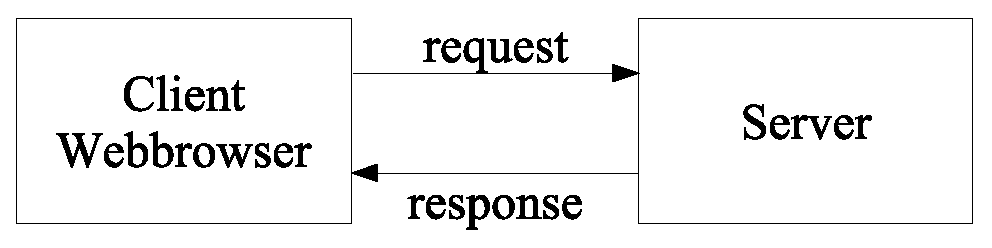
\includegraphics[width=10cm]{images/request_cycle.eps}
      \caption{Request-Anfrage vom Client an Server}
      \label{fig:request_cycle}
    \end{figure}
    
    
  \section{Kategorien von Webanwendungen}
  
    Webanwendungen besitzen unterschiedliche Komplexit�ten. Sie reichen von 
    einfachen Informationsseiten bis zu komplexen Programmabl�ufen. 
    Nach \cite{defwebappl} werden folgende Kategorien von Webanwendungen unterteilt:
    
    \label{webkategorien}
    \begin{itemize}
      \item Dokumentenzentriert \\
            Hier werden fertige Dokumente auf dem Server gelegt und bei Anfrage 
            als Antwort ausgegeben. Beispiele sind einfache Firmenpr�sentationen oder das Webradio.
      \item Interaktiv \\
            Hier hat der Anwender die M�glichkeit �ber einfache Interaktionen die 
            Webanwendungen zu steuern. Dies kann z.B. durch eine einfache 
            HTML-Formular-Technik und durch die Link-Technik 
            umgesetzt sein.
      \item Transaktional \\
            Durch ein Datenbanksystem kann eine konsistente Datenhaltung 
            erreicht werden. Ein Beispiel daf�r ist ein Resevierungssystem.
            Daten sind nicht nur �ber eine Session bekannt, sonder werden
            dauerhaft gespeichert.
      \item Workflow-basiert \\
            Diese erlauben Abwicklungen von Gesch�ftsprozessen intern oder zwischen verschiedenen
            Teilnehmern. Daf�r sind Web-Services mit definierten Schnittstellen notwendig.
            Beispiele sind Business-to-Business-L�sungen (B2B) im 
            E-Commerce-Bereich oder E-Government-Anwendungen im
            Bereich der �ffentlichen Verwaltung.
      \item Kollaborativ \\
            Hier werden die Webanwendung zur Kooperation bei unstrukturierten Vorg�ngen und 
            hohem Kommunikationsbedarf verwendet. Beispiel daf�r sind  Chatrooms und 
            gemeinschaftliche Arbeitsr�ume um gemeinsame Informationen generiereren, bearbeiten
            und verwalten zu k�nnen (z.B. Wikipedia).\\
            \\
      \item Portalorientiert \\
            Diese vereinen den Zugriff auf verteilte und verschiedenen Informationsquellen und 
            Informationsdienste unter einer einheitlichen Oberfl�che
            (Single Point of Access).
      \item Ubiquit�r \\
            Stellen personalisierte Dienste zu jeder Zeit, an jedem Ort und 
            f�r eine Vielzahl von Endger�ten zur Verf�gung.  
      \item Semantisches Web \\
            Informationen im Web sollen nicht nur f�r den Menschen verst�ndlich 
            aufbereitet, sondern auch f�r Maschinen automatisch verarbeitbar 
            gemacht werden. Dadurch kann neues relevantes Wissen automatisch 
            ermittelt werden. Dies wird bei Recommender-Systeme eingesetzt
             um z.B. Kunden Produkte zu empfehlen oder ihnen f�r ihre Kaufentscheidung 
             hilfreiche Informationen zur Verf�gung zu stellen. 
    \end{itemize}
    
    In der Praxis gibt es keine so strikte Trennung f�r die Webanwendungen, sondern 
    es werden verschiedene Mischformen vorhanden sein.  
    
  \section{Darstellungsm�glichkeiten von Webanwendungen}

    Nachdem wir gekl�rt haben, was Webanwendungen sind, sollen im Folgenden 
    die gebr�uchlichsten Darstellungsm�glichkeiten von Webanwendungen 
    beschrieben werden. 
    \begin{itemize}
      \item HTML und HTML mit CSS\\
            HTML ist eine Seitenbeschreibungssprache, die vom W3C standardisiert wurde. Die
            aktuelle Version ist 4.0. Alle Browser unterst�tzen HTML 4.0. Leichte 
            Darstellungsunterschiede gibt es dennoch zwischen den Browsern. Mit CSS k�nnen die 
            Formatierungsinformationen von den Daten und die Grundstruktur der Webseite getrennt werden.
            Dies ist ein Schritt zur Trennung von Inhalt und Darstellung. 
      \item XHTML \\
            XHTML entspricht im Wesentlichen HTML, die 
            Dateien m�ssen allerdings XML-konform sein. Dies wurde in HTML noch nicht konsequent 
            durchgesetzt.
            Der Vorteil von XHTML gegen�ber HTML ist, das XML-Werkzeuge zur Syntax�berpr�fung gut 
            geeignet sind.
      \item HTML mit Javascript \\
            Javascript wird clientseitig ausgef�hrt, d.h. der Client muss den Befehlsatz von Javascript 
            interpretieren k�nnen. Javascript wurde von Netscape entwickelt und als offener Standard f�r eine
            Objekt-Skriptsprache bezeichnet. Leider wurde Javascript nicht vom W3C standardisiert. Als
            Gegenprodukt von Microsoft wurde JScript eingef�hrt. Javascript und JScript sind sehr �hnlich, 
            aber doch nicht
            gleich. Darum gibt es sehr viele Inkompatibilit�ten zwischen den Browsern, weshalb 
            Javascript nur bedingt
            in Webanwendungen verwendet werden sollte. Der Vorteil von Javascript ist, 
            dass schon clientseitig auf 
            Benutzereingabe reagiert werden kann, ohne den Server zu befragen und dadurch Interaktionen ohne 
            kompletten Neuaufbau des Frames realisierbar sind.
      \item XML mit XSLT \\
            Hier wird die Trennung von Inhalt und Darstellung umgesetzt. In der XML-Datei stehen die ganzen
            Daten 
            f�r die Darstellung und in der XSLT-Datei die ganzen Formatierungen und Strukturierungen f�r 
            die Darstellung der Daten. Auf den Server werden diese zwei Dateien zusammengebracht und
            das Ergebnis wird zum Client (Browser) geschickt. 
      \item Serverseitige Skriptsprache (PHP, CGI, ...) \\
            Diese Skriptsprachen werden auf dem Server ausgef�hrt und das Ergebnis wird zum Browser geschickt. In
            ihnen k�nnen komplexe Anwendungslogiken hinterlegt werden. Dies ist auch der Vorteil
            der Skriptsprachen, weil damit komplexe Webanwendungen realisierbar sind. 
            Man greift auf die 
            vielen vorgefertigten Bibliotheken, die in den Skriptsprachen schon enthalten sind, zur�ck, so dass
            Standardwebanwendungen relativ z�gig entwickelbar sind. F�r die Trennung von Darstellung und
            Anwendungslogik k�nnen hier Template-Systeme verwendet werden.\\
            \\
      \item Serverseitige Anwendungssprachen (Servlet, ASP, JSP, ...) \\
            Diese werden auf dem Server ausgef�hrt. Im Unterschied zu den serverseitigen
            Skriptsprachen sind sie in einer Programmiersprache wie Java, Visual Basic usw.
            geschrieben und liegen auf dem Server in einer kompilierten Form vor
            (Servlets) oder werden zur Laufzeit kompiliert (JSP) und danach ausgef�hrt.
    \end{itemize}
    Auch hier sind wieder Mischformen vorhanden und denkbar. Ein Beispiel daf�r ist die 
    Fehler�berpr�fung von Eingaben 
    durch Javascript und die Ausf�hrung der restlichen Anwendungslogik durch
    serverseitige Skriptsprachen oder serverseitige Anwendungssprachen.
    
  \section{Einordung von CYBOP}
  
    Zurzeit 
    k�nnen dokumentenbasierte und interaktive Webanwendungen mit CYBOP erstellt werden.
    Ein Beispiel f�r eine interaktive Webanwendung ist der Prototyp, der im Rahmen der
    Diplomarbeit entstanden ist. Der n�chste Schritt f�r CYBOP ist die Umsetzung von 
    transaktionalen Webanwendungen. Dazu ist die Abspeicherung von Daten in 
    persistenten Medien notwendig. 
  
    Als Darstellung kommen aus Architekturgr�nden  nicht alle 
    m�glichen Formen in Frage. Alle serverseitigen 
    fallen heraus, da CYBOP mit seinen Komponenten 
    bereits eine serverseitige Architektur darstellt. Also 
    sind nur clientseitige Darstellungsm�glichkeiten wie HTML, XHTML
    und Javascript in Betracht zu ziehen. HTML ist zwar standardisiert, hat aber noch viele
    Freir�ume bez�glich von Schreibweisen. In dieser Beziehung ist XHTML die bessere
    Wahl, da hier die Wohlgeformtheit von XML-Dokumenten eingehalten werden muss.
    Dadurch sind die Strukturen f�r die Generierung besser definiert und es
    m�ssen nicht so viele Ausnahmebedingungen in CYBOI integriert werden.
    Javascript ist keine unabh�ngige Technologie, sonder von einer Firma abh�ngig. 
    Es wird zwar  von vielen g�ngigen Webbrowsern unterst�tzt, ist aber nicht 
    standardisiert. Damit ist diese Technologie f�r CYBOP nicht zu empfehlen.
    F�r die Umsetzung in CYBOP bleibt nur die eine sinnvolle Darstellungsm�glichkeit, XHTML,
    �brig. 
  
    
    


  \chapter{Webserver und dessen Integration in CYBOI}

  \section{Hintergrund}
  
    
    Zur Beantwortung einer Anfrage eines Clients an einen Server �ber das  
    Http-Protokoll ist ein Webserver n�tig.
    Dies kann durch einen vorhandenen Webserver, wie z.B. Apache, oder durch einen selbst 
    programmierten Webserver realisiert werden. Dieser Webserver muss f�r CYBOL
    angepasst werden. Bei einem bestehenden Webserver ist eine Erweiterung 
    z.B. durch ein CYBOI-Plugin m�glich. Der Vorteil der Erweiterung eines bestehenden Webservers
    ist die Verwendung der ganzen Funktionalit�t, wie z.B. die Session-Verwaltung und 
    die Skalierbarkeit. Das Hauptproblem bei der Integration
    w�re die Anpassung der verschiedenen Softwarearchitekturen (bestehender Webserver und CYBOI).   
    Ein weiterer Nachteil ist die Abh�ngigkeit des Plugins zu einem bestehenden 
    Webserver, das bedeutet dass bei �nderungen des Webservers auch das Plugin anzupassen ist.
    Die Kontrolle w�rde nicht allein beim CYBOP-Projekt liegen. 

    Da die Implementierung f�r CYBOL insgesamt als Prototyp geplant ist, reicht es aus,
    einen kleinen Webserver selbst zu programmieren, so dass man 
    die gesamte Verf�gungsgewalt �ber das Projekt 
    und dessen Quelltext hat. Weiterhin kann im Softwaredesign eine bessere Homogenit�t erreicht werden.
    �nderungen am Webserver sind somit leichter zu realisieren. Der Nachteil ist hier, das die
    Standardfunktionalit�t von Webservern, wie z.B. die Session-Verwaltung, in CYBOI 
    programmiert werden muss. 
    
    Die Vorraussetzungen f�r einen Webserver sind die Sockets. Diese stellen die 
    Kommunikationsschnittstelle zwischen den einzelnen Komponenten dar. Wichtiger 
    Bestandteile f�r die Integration des Webserver-Prototyps in CYBOI
    sind Prozesse und Threads. Da bei der Implementierung der Sockets blockierende
    Sockets verwendet werden, 
    %\(siehe Abschnitt ref{{blocksocktets}), 
    ist es notwendig
    den Webserver in einem eigenen Prozess bzw. Thread laufen zu lassen. 
    
      \section{Sockets}  
  
     Sockets sind nach \cite{defsockets} folgenderma�en definiert. 
    \begin{quotation}
      Sockets is a method for communication between a client program and a server program in a network. 
      A socket is defined as the endpoint in a connection. Sockets are created and used with a set 
      of programming requests or function calls sometimes called the sockets application 
      programming interface (API). The most common sockets API is the Berkeley UNIX C language 
      interface for sockets. Sockets can also be used for communication between processes 
      within the same computer. 
    \end{quotation}
    
    Ein Socket ist also eine Schnittstelle zwischen einem Prozess 
    und einem Transportprotokoll. Letzteres kann z.B. TCP oder UDP sein. 
    Das Socket-Prinzip entspricht dem von File-Deskriptoren. 
    Dort repr�sentiert nach dem �ffnen einer Datei ein Handle die Verbindung
    zu dieser Datei und unter Angabe des Handles ist der Lese- oder Schreibzugriff m�glich. 
    Bei Sockets geht es jedoch nicht um physikalische Dateien sondern um Kommunikationskan�le, �ber 
    die Daten gesendet und empfangen werden k�nnen.

    Socket-Schnittstellen sind zwar von keiner Institution genormt, 
    stellen aber einen de-facto- bzw. Industriestandard dar, was zum einen daran liegen d�rfte, 
    dass sie leicht verst�ndlich sind, zum anderen f�gen sie sich ausgesprochen 
    harmonisch in die UNIX-Umwelt ein. Eine Variante der Socket-Schnittstelle wurde von 
    Microsoft und verschiedenen anderen Firmen unter der Bezeichnung WinSock in das 
    Schnittstellenangebot der Windows Open Service Architecture (WOSA) aufgenommen und 
    d�rfte damit auch ein etablierter Standard in der PC-Welt sein.
    
    \subsection{Arten von Sockets}
    
      Sockets stellen eine allgemeine Form der Kommunikation zwischen Dateien, Prozessen usw. dar.
      Schon allein die Verwendung unterschiedlicher �bertragungsprotokolle 
      spezifiziert unterschiedliche Anwendungsgebiete. 
      Folgende Arten von Sockets werden darum unterschieden:
      
      \begin{itemize}
        \item Stream Socket \\
              Stream Sockets setzen auf dem verbindungsorientierten TCP auf. Er ist
              langsamer als ein Datagramm Socket, aber daf�r wird die �bertragungskontrolle 
              gew�hrleistet.
        \item Datagram Socket \\
              Datagram Sockets setzen auf dem verbindungslos orientierten User Datagram Protocol (UDP) auf.
              Das gro�e Problem dabei ist, dass die �bertragungskontrolle fehlt. Ansonsten ist die 
              �bertragungsart sehr schnell, falls die Pakete ankommen und erzeugt kaum
              Overhead.
        \item Raw Socket \\
              Ein Raw Socket ist ein spezieller Socket. Er erm�glicht dem Benutzer den 
              direkten Zugang zum Netzwerk, 
              indem man eigene Pakete einspeisen kann. Raw Socket benutzen z.B. das Protokoll ICMP. 
              Sie sind sehr 
              schnell, da sie auf eine tiefere Protokollfamilie aufsetzen und damit weniger Overhead haben. 
        \item Unix Domain Sockets \\
              Unix verwendet Sockets zur lokalen Interprozess-Kommunikation, sog. Unix Domain Sockets. 
              Sie sind Teil des POSIX-Standards. Dies ist die urspr�ngliche Form des 
              von BDS entwickelten Sockets.
      \end{itemize}
  
      F�r den Webserver der vorliegenden Diplomarbeit wird ein Stream Socket mit dem Protokoll TCP verwendet.  
      Da in einer Anwendung sichergestellt werden muss, das die Datenpakete ankommen und 
      auch in der richtigen Reihenfolge zusammengesetzt werden, ist nur ein Stream Socket mit der 
      entsprechenden �bertragungskontrolle verwendbar.

    \subsection{Arbeitsweise von Sockets}
    
      Sockets arbeiten immer nach einen bestimmten Muster. Als erstes ist der Server f�r die
      Bearbeitung des Sockets vorzubereiten. Dazu muss er veranlasst werden �ber einen bestimmten
      Port auf die Anforderungen der Clients zu warten. Ports geh�ren zu der Adresskomponente 
      einer Netzwerkkommunikation. Der Port ist mit 16 Bit kodiert. Damit kann der Port Werte von 
      0 bis 65535 annehmen. Die Ports bis zur 1024 sind f�r verschiedenen Dienste (FTP, HTTP, ...)
      definiert. Die Portnummern h�her als 1024 stehen zur freien Verf�gung, wobei sich auch hier schon
      f�r gewisse Dienste  Standard-Portnummern eingeb�rgert haben. 
      
      In der Abbildung \ref{fig:tcpsocket} ist einen typischen Ablauf eines Stream Sockets zu sehen.
      \begin{figure}[H]
        \centering
          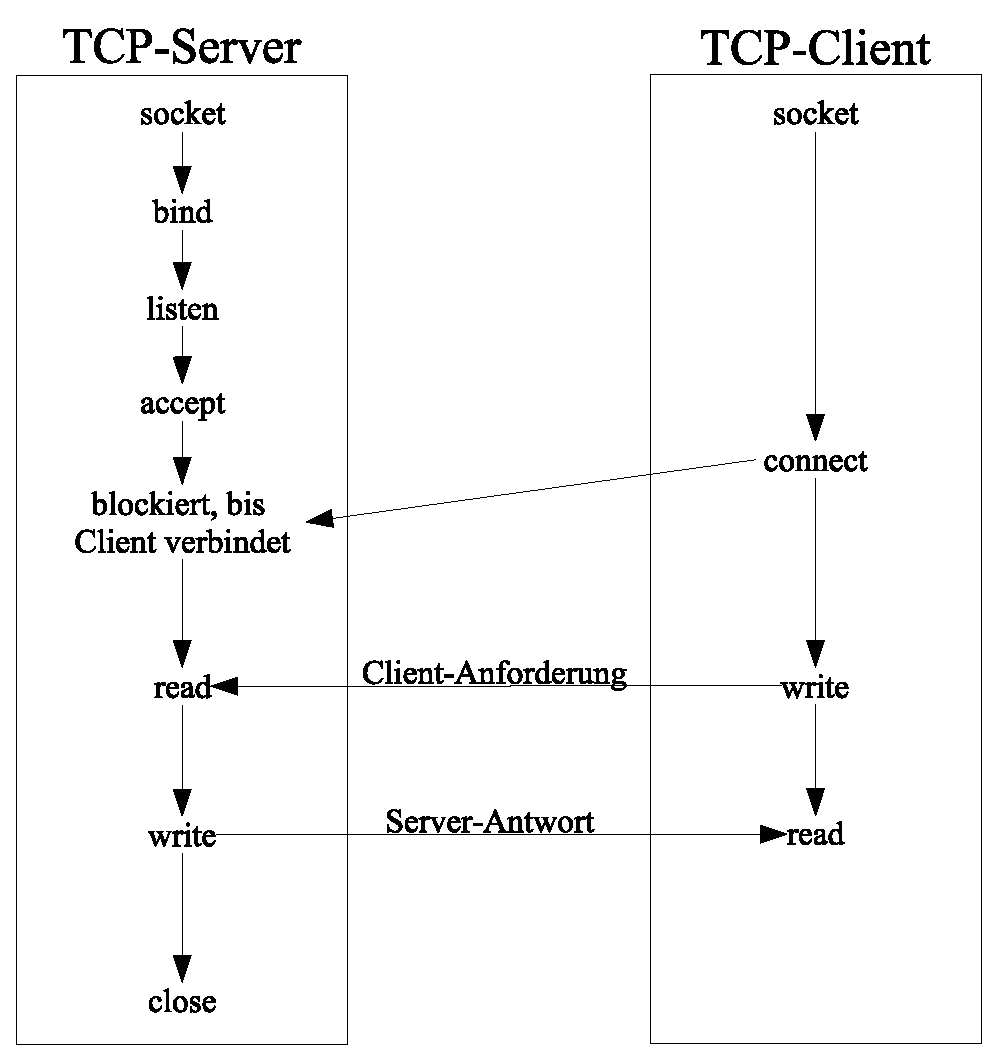
\includegraphics[width=10cm]{images/tcpsocket.eps}
        \caption{Ablauf TCP-Socket}
        \label{fig:tcpsocket}
      \end{figure}
      Als erstes muss der Socket erstellt werden. Mit \emph{bind} wird dieser Socket 
      an eine bestimmte Portnummer gebunden und mit dem Befehl \emph{listen} wird 
      dem Socket mitgeteilt, das er auf Verbindungsversuche zu dieser Portnummer 
      lauschen soll. Jetzt wartet der Server mit \emph{acceppt} auf einen 
      Verbindungsversuch des Clients. Dies ist entweder als blockierende oder
      nicht blockierende Funktion implementiert (siehe Abschnitt \ref{blocksocktets}). 
      Nach dem \emph{accept} die Verbindung akzeptiert hat, wird der normale
      Kommunikationsprozess durchgef�hrt. Als erstes liest der Server (\emph{read}) die Anfrage
      vom Client und schickt eine Antwort (\emph{write}) an den Client zur�ck.
      Danach ist vom Server die Verbindung zu beenden (\emph{close}).


    \subsection{Blockierende und nicht blockierende Sockets}
      \label{blocksocktets}  
  
      Gewisse Funktionen einer Socketoperation k�nnen als blockierende oder nicht blockierende 
      Operation ausgef�hrt werden. Blockierend bedeutet, dass die Funktion so lange wartet,
      d.h. dass das restliche Programm an dieser Stelle unterbrochen wird, 
      bis die Aktion ausgef�hrt wurde. Eine typische Operation ist das Warten auf eine
      Anfrage vom Client. In dieser Zeit ist der Prozess stillgelegt, bis eine Anfrage 
      auf dem Kommunikationskanal anliegt. So lange der Prozess wartet, wird keine
      Prozessorleistung verbraucht. Andere Prozesse auf 
      dem Rechner k�nnen normal weiterarbeiten, da der Prozessor keine Belastung durch das
      Warten auf eine Anfrage hat. Wenn diese Operation als nicht blockierende 
      Operation realisiert w�re, so w�rde, wenn kein Anfragesignal auf dem 
      Kommunikationskanal anliegt, die Funktion an dieser Stelle nicht warten, sondern einfach 
      im Programm weitermachen. Um nun eine Anfrage �ber das Socket zu registrieren, ist die Ausf�hrung 
      der Operation in einer Endlosschleife n�tig. Dies verbraucht aber viele Ressourcen des Prozessors.
      Auf Grund der Performance des Gesamtsystems sind also blockierende Sockets vorzuziehen.

    
    \section{Prozesse und Threads}

  Da die Implementierung des Webservers mit blockierenden Sockets erfolgt, ist
  es erforderlich, parallele bzw. nebenl�ufige Programme in CYBOI zu starten, 
  da ansonsten die blockierenden Socketoperationen den gesamten
  Interpreter CYBOI lahm legen. Es gibt zwei M�glichkeiten parallele bzw. nebenl�ufige 
  Programme zu starten, entweder als eigenst�ndiger Prozess oder 
  als Thread. F�r die Auswahl sind beide Varianten zu erkl�ren und Vor- und Nachteile 
  gegen�berzustellen. 
     
  \subsection{Prozess}
   
    Ein Prozess aus Betriebssystemsicht ist ein in Ausf�hrung befindliches Programm,
    welches sequentiell abgearbeitet wird. Es wird immer nur
    eine Instruktion zu einer bestimmten Zeit ausgef�hrt. Ein Prozess besteht
    aus dem Programm und der Programmumgebung und er verf�gt �ber einen
    eigenen Adressraum. Zu der Programmumgebung geh�ren Programmz�hler, 
    alle Registerinhalte, Stack (tempor�re Daten) und der Datenbereich (globale Variablen).
    Da das Betriebssystem mehrere Prozesse
    gleichzeitig verwaltet und es so aussieht, als ob die Prozesse parallel ablaufen, 
    m�ssen diese Prozesse verschieden Zust�nde annehmen k�nnen. Folgendes Bild veranschaulicht die
    Prozesszust�nde und welche Wechsel zwischen den Prozesszust�nden m�glich sind.
  
    \begin{figure}[H]
      \centering
        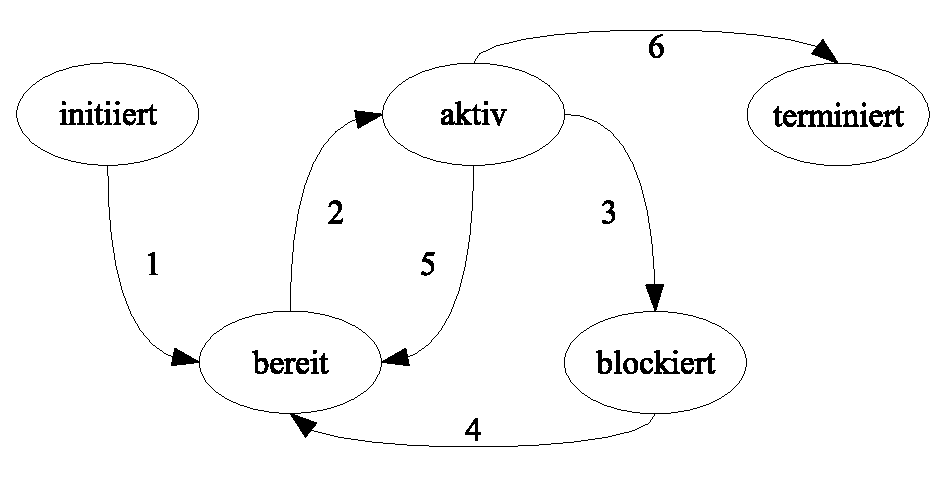
\includegraphics{images/prozeszustaende.eps}
      \caption{Prozesszust�nde}
      \label{fig:prozeszustaende}
    \end{figure}

    Als erstes wird ein Prozess initiiert. Dazu werden alle Initialbetriebsmittel
    alloziiert (1). Danach ist der Prozess in dem Zustand \emph{bereit}. In diesem Zustand kann der Prozess
    noch nichts machen, da ihm noch keine Prozessorzeit zugeordnet ist. Dies wird durch
    den Prozessscheduler des Betriebssystems realisiert (2). Dieser Scheduler kann den Prozess
    auch wieder in den Zustand \emph{bereit} zur�ckversetzen (5). Dies kann z.B. durch Ablauf der Zeitscheibe 
    oder durch Priorit�tensteuerung passieren. Wird von einem aktiven Prozess ein
    Betriebsmittel angefordert und dieses ist zurzeit nicht verf�gbar, so wird der Prozess 
    in den Zustand blockiert gesetzt (3). Liegt ein Signal an, dass das erwartete Betriebsmittel 
    zur Verf�gung steht,
    so wechselt der Status des Prozesses in den Zustand \emph{bereit} (4).
    Am Ende wird der Prozess abgeschlossen und alle Betriebsmittel und Ressourcen werden freigegeben. 
    
    Um zwischen den Prozessen umschalten zu k�nnen, m�ssen Informationen des Prozesses gesichert werden.
    Dazu dienen so genannte Prozess-Kontroll-Bl�cke (PKB). Diese beinhalten folgende Informationen:
    \begin{itemize}
      \item Prozesszustand
      \item Zeiger auf Prozess
      \item Prozess-Id
      \item Programmumgebung
      \begin{itemize}
        \item Programmz�hler
        \item Prozessorregister
        \item I\/O Statusinformationen
         \item Speicherverwaltungsinformationen
      \end{itemize}
    \end{itemize}
    Um nun von einen zum anderen Prozess zu wechseln, wird der gesamte PKB gesichert 
    und der PKB vom aktivierten Prozess geladen. Diese Art von Prozessen wird auch als 
    Single-Thread-Prozessor-Modell bezeichnet.
    \begin{figure}[H]
      \centering
        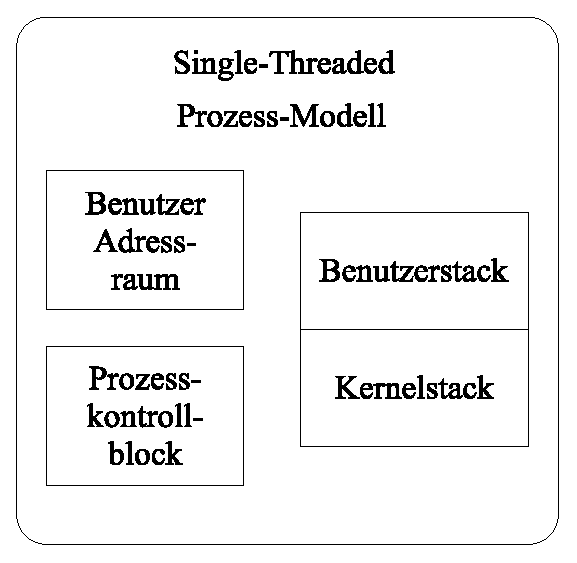
\includegraphics{images/singlethreadprozess.eps}
      \caption{Single-Thread-Prozess-Modell}
      \label{fig:singlethreadprozess}
    \end{figure}
    
   Ein Prozess kann weitere Unterprozesse
   generieren, so dass eine Baumstruktur von Prozessen und ihren Unterprozessen
   entsteht. Die Umschaltung zwischen den Prozessen (siehe vorheriges Kapitel) erfordert
   die Sicherung und das Laden des gesamten Prozess-Kontroll-Block und der Stacks. 
   
  \subsection{Parallele und nebenl�ufige Prozesse}
  
   Ein Prozess wird sequentiell im Prozessor abgearbeitet. Richtige parallele
   Arbeitung von Prozessen gibt es nur in Mehrprozessorrechnern. In 
   Einprozessormaschinen gibt es keine echte parallele Verarbeitung, sondern
   nur eine nebenl�ufige (quasi parallel) Abarbeitung von Prozessen. 
   Dies wird durch das Betriebssystem intern geregelt. 
   Da es f�r den 
   Endanwender keinen Unterschied bedeutet, ob nebenl�ufige oder parallele Abarbeitung vorliegt, 
   wird nur noch auf nebenl�ufige Prozesse eingegangen.

\newpage  
   Hier eine Definition f�r nebenl�ufige Prozesse:
   \begin{quotation}
     Zwei oder mehrere Prozesse werden als nebenl�ufig bezeichnet, wenn sie weitgehend unabh�ngig 
     vom Betriebssystem bearbeitet werden k�nnen. Dabei spielt es keine Rolle, 
     ob sie von einem Multiprozessor-System parallel bearbeitet werden oder ihre 
     Abarbeitung sequentialisiert werden, d.h. sie werden in einer durch 
     das Betriebssystem bestimmten Reihenfolge abgearbeitet. Dabei ist es auch m�glich, 
     dass ein Prozess w�hrend der Bearbeitung unterbrochen wird, dann ein anderer 
     bearbeitet und der abgebrochene erst nach einer Verweildauer fortgesetzt wird. 
     Man muss zwischen unabh�ngigen nebenl�ufigen Prozessen, bei denen das Ergebnis 
     nicht von der Abarbeitungsreihenfolge abh�ngig ist, und abh�ngigen nebenl�ufigen Prozessen, 
     bei denen eine Synchronisation notwendig ist, unterscheiden. Betriebssysteme gehen in 
     der Regel davon aus, dass die Prozesse unabh�ngig von einander sind. Sind Prozesse von einander
     abh�ngig, so m�ssen sie synchronisiert werden.  
   \end{quotation}
   
     
   \subsection{Threads}
 
     Als Thread wird ein leichtgewichtiger Prozess bezeichnet, der nur die wichtigsten Kontextinformationen 
     mit sich f�hrt. Im Prinzip werden innerhalb eines Prozesses mehrere Threads gehalten. Diese
     Threads teilen sich den Benutzer-Adressraum. Dadurch 
     wird ein Wechsel zwischen verschiedenen Threads leichter. So k�nnen innerhalb einer 
     Anwendung mehrere Teilprozesse nebenl�ufig ausgef�hrt werden. 
     Die Abbildung \ref{fig:multithreadprozess} verdeutlicht die gemeinsame Nutzung vom 
     Benutzer-Adressraum und das Ausf�hren von mehreren Threads innerhalb eines Prozesses.
    \begin{figure}[H]
      \centering
        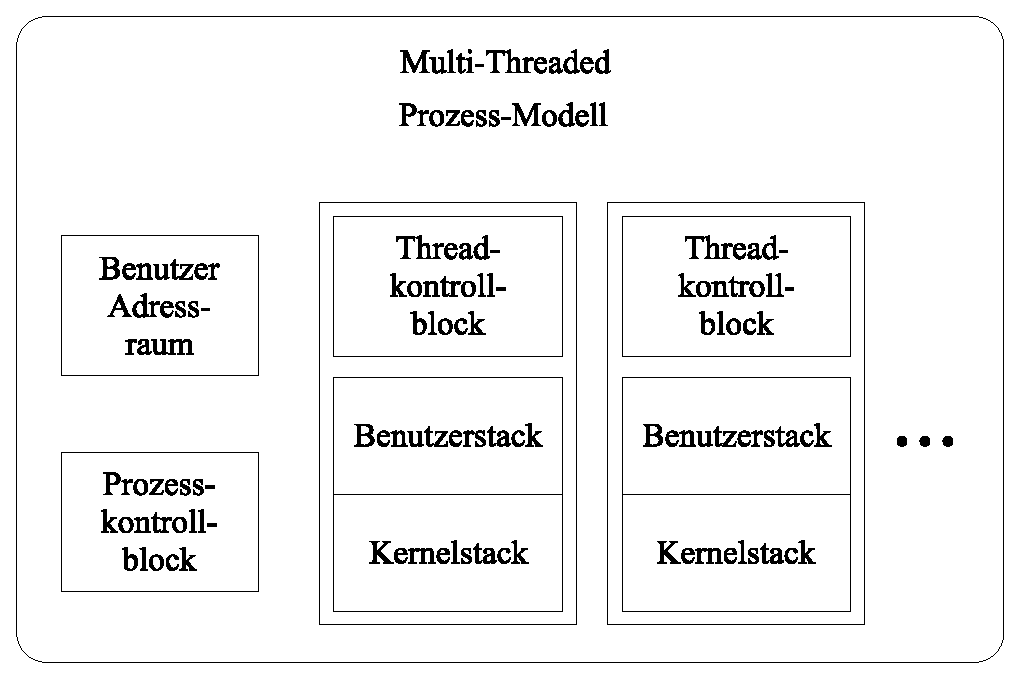
\includegraphics[width=10cm]{images/multithreadprozess.eps}
      \caption{Multi-Thread-Prozess-Modell}
      \label{fig:multithreadprozess}
    \end{figure}
    Der Interpreter CYBOI wird in C geschrieben. Dieser Quelltext wird unter Linux kompiliert 
    und ausgef�hrt. Eine M�glichkeit f�r Windows w�re \emph{cygwin}, das die kompletten GNU-Tools
    und Bibliotheken auch f�r Windows zur Verf�gung stellt. Die C-Bibliothek pthread 
    hat sich f�r die Threadbehandlung etabliert. In dieser Bibliothek sind M�glichkeiten zur 
    Erzeugung, Beendung und Synchronisation von Threads vorhanden.
     
  \subsection{Vergleich Threads und Prozesse}
   
    F�r die Integration des Webservers in CYBOI wurden die leichtgewichtigen Prozesse
    (Threads) ausgew�hlt. Da Threads innerhalb eines Prozesses von sich aus den gleichen Adressraum
    verwenden, ist eine direkte Kommunikation zwischen CYBOI und den Webserver �ber den
    gleichen Adressraum m�glich, womit bei Threads die Kommunikation �ber andere aufwendigere
    Kommunikationskan�le entf�llt. Ein weiterer Vorteil ist die Geschwindigkeit der Operationen von Threads.
    Da weniger Informationen involviert sind, sind die Operationen f�r Threads
    auch schneller als bei Prozessen. Dies betrifft sowohl die normalen Operationen, wie z.B. Aktivieren,
    Erzeugen, Blockieren als auch den Kontextwechsel zwischen den Threads. 
    Die Nachteile von Threads sind, dass dem Betriebssystem die Kontrolle �ber die Threads
    entzogen ist. Der Entwickler muss selbst darauf achten, dass sich diese nicht gegenseitig
    blockieren. Weiterhin ist durch die Benutzung des gleichen Adressraumes nicht der Schutz
    vor anderen Threads gesichert. Dieser ist ebenfalls vom Entwickler sicherzustellen. 
    
\section{Synchronisation von Threads}

  Die Kommunikation von Threads erfolgt �blichweise �ber den gemeinsamen 
  Benutzer-Adressraum. Da Threads nebenl�ufig arbeiten, m�ssen die Zugriffe auf gemeinsame Variablen 
  synchronisiert werden, da es ansonsten zu Kollisionen beim gleichzeitigen Zugriff 
  auf den gemeinsamen Speicherbereich kommen kann. Die pthread-Bibliothek stellt daf�r 
  zwei M�glichkeiten zur Verf�gung, entweder �ber Mutex oder mit Bedingungsvariablen.


  \subsection{Threadsynchronisation mit Mutex}

    Mutex ist ein Kunstwort, welches sich aus den W�rtern MUTual und EXclusions (gegenseitiger Ausschluss) 
    zusammensetzt. Sie dienen dazu, Ressourcen f�r Threads exklusiv zu reservieren. 
    Dabei kann ein Mutex immer nur von einem Thread belegt sein. Versuchen weitere Threads diesen Mutex f�r 
    sich zu beanspruchen, werden diese blockiert, bis der aktuelle Besitzer den Mutex wieder freigibt. 
    Da die Belegung atomar erfolgt, ist auch sichergestellt, dass immer nur ein Thread einen Mutex 
    zur selben Zeit belegt. Mutex liegt das Semaphoren-Konzept zu Grunde.
    
    Semaphor im Allgemeinen bedeutet, dass ein Zugriff auf einen kritischen Bereich (Shared memory) 
    gesch�tzt wird. Dazu besteht ein Semaphor aus zwei Elementen, dem Semaphor-Wert s(ganzzahlig) 
    und einer Warteschlange. Ist der Semaphoren-Wert gr��er Null, so bedeutet dies, 
    dass der kritische Abschnitt 
    betreten werden kann. Ansonsten ist der Abschnitt durch einen anderen Prozess belegt. 
    Die Warteschlange dient zur Speicherung aller Prozesse, die nicht den kritischen Abschnitt 
    betreten konnten.
    Zum weiteren sind f�r Semaphoren zwei Operationen P(s) und V(s) folgenderma�en definiert.
    \\ \\
    \verb|    P(s):  s = 0 | $\rightarrow$ Prozess in Warteschlange schlafen legen
    \\
    \verb|           s > 0 | $\rightarrow$ s um eins erniedrigen
    \\
    \verb|    V(s): | $\rightarrow$ s um eins erh�hen
    \\
    \verb|          | $\rightarrow$ falls Warteschlange nicht leer ist, so n�chsten Prozess aufwecken
    \\ \\
    Ein bin�rer Semaphore ist ein normaler Semaphor mit Initialisierung der 
    Semaphoren-Variable auf eins. Mutexe stellen bin�re Semaphoren dar, wobei die 
    Implementierung ohne die Warteschlange realisiert wurde.  
    
    Das Prinzip von Mutex ist einfach. Ein Thread arbeitet mit einer globalen oder 
    statischen Variable, die f�r allen anderen Threads w�hrend einer Operation 
    von einem Mutex blockiert 
    (gesperrt) wird. Ben�tigt der Thread diese Variable nicht mehr, gibt er diese frei.
    Durch das Setzen der Sperren im Programm liegt die Verantwortung einer 
    Verklemmungsfreiheit  beim Programmierer.
    Dadurch k�nnen aber bei unsauberer Programmierung Deadlocks auftreten, falls
    ein Thread die Sperrung nicht ordnungsgem�� freigibt oder es Ressourcen anfordert, 
    obwohl es schon Ressourcen bekommen hat.
     
  \subsection{Threads synchronisieren mit Bedingungsvariablen}
  
  
    Die Bedingungsvariablen dienen dazu, den Eintritt bestimmter Bedingungen abzuwarten 
    beziehungsweise deren Erf�llung anzuzeigen und k�nnen dazu genutzt werden
    Threads zu synchronisieren. Bedingungsvariablen sind an Mutexe gekoppelt um 
    sicherzustellen, dass die Bedingungen immer nur von einem Thread zu einer 
    Zeit ge�ndert werden k�nnen. 
    In der folgenden Abbildung ist das Prinzip der \emph{Condition Variable} zu erkennen.
    Dies ist aus dem Buch \cite{linuxprog} entnommen.
    \begin{figure}[H]
      \centering
        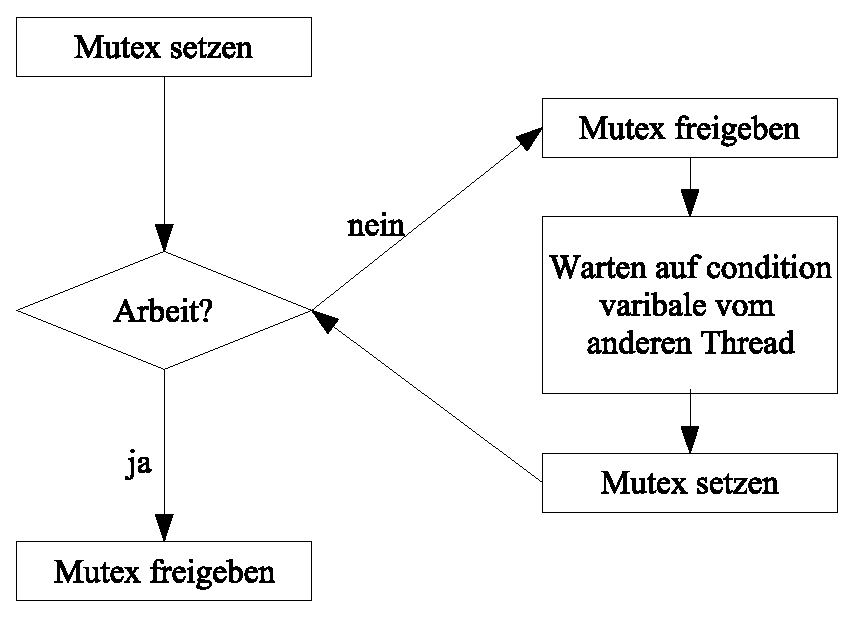
\includegraphics[width=10cm]{images/condvar.eps}
      \caption{Condition Variable}
      \label{fig:condvar}
    \end{figure}
    Am Anfang wird ein Mutex f�r einen kritischen Bereich gesetzt. Kann der Thread 
    nicht weiter arbeiten, weil zum Beispiel die ben�tigen Daten nicht anliegen, so
    wird dieser stillgelegt. Der Mutex wird freigegeben, es wird gewartet 
    bis diese Bedingung (Daten vorhanden) eintrifft und danach der Mutex wieder belegt. 
    Dies ist alles in einer Funktion der pthread-Bibliothek gekapselt. 
    Danach kann der Thread ganz normal seinen kritischen Bereich abarbeiten 
    und den Mutex wieder freigeben.

  \subsection{Fazit der Synchronisation}
  
    Die zwei vorgestellten Synchronisationsarten schlie�en sich nicht aus, sondern erg�nzen sich.
    Mutex ist f�r den einfachen gegenseitigen Ausschluss da. Dieser Mechanismus wird bei den 
    Bedingungsvariablen auch genutzt. Welche Form der Synchronisation ist f�r
    die Integration vom Webserver in CYBOI notwendig? Dazu ist die zu l�sende Aufgabe
    n�her zu betrachten. Wird im Webserver eine Anfrage vom Client gestellt, so ist ein Signal im
    \emph{Signal Memeory} zu erstellen. Dieses Signal ist die Umwandlung der Anfrage vom Client
    in die interne Repr�sentation von Signalen in CYBOI. Dazu ist es einfach nur notwendig, 
    die Variable \emph{Signal Memory} f�r den gegenseitigen Ausschluss zu sichern. Also ist 
    es ausreichend, die Synchronisation mit Mutex zu realisieren. 

  \chapter{Umsetzung der praktischen Aufgabe}

  \section{�berblick}
    
    Als praktisches Ergebnis dieser Diplomarbeit soll ein Prototyp 
    erstellt werden, der die M�glichkeit der Umsetzung von 
    einer Webanwendung mit CYBOP aufzeigt. Dazu wurde das Beispiel
    einer kleinen Adressverwaltung gew�hlt, wo die Adressen
    editierbar, l�schbar und neu anlegbar sind. 
    
  
  \section{Anpassung von CYBOL}
  
    Als erstes musste im Rahmen der Diplomarbeit in Zusammenarbeit mit Christian Heller die 
    Spezifikation der Beschreibungssprache auch hinsichtlich der Webanwendungsf�higkeit 
    fertig gestellt werden. Dabei mussten sowohl allgemeine als 
    auch webspezifizische Sprachkonstrukte ber�cksichtigt werden. Es wurde 
    festgestellt, dass der prinzipielle Aufbau von CYBOL die Belange 
    von webspezifischen Anforderungen ohne Probleme erf�llt. 
    Erweiterungen mussten nur in den Auspr�gungen der Werte, wie z.B. die  neue 
    Operation \emph{url\_refresh}, die zur Zeit nur im Web Sinn macht, oder verschiedene
    Properties, die f�r die Generierung von XHTML-Seiten von Bedeutung sind, vorgenommen werden.
    
    Im Folgenden m�chte ich kurz auf die Elemente von CYBOL eingehen, die
    f�r den Prototyp der Diplomarbeit relevant sind. Dazu geh�ren welche Arten von 
    \emph{channel} und \emph{abstraction} verwendet werden und welche Operationen definiert und
    programmiert werden mussten, damit diese Anwendung technisch umgesetzt werden konnte.
    
    F�r \emph{channel} werden hier nur zwei Arten verwendet. Vorgesehen sind weitere 
    Kommunikationskan�le. Diese sind aber noch nicht umgesetzt.
    \begin{table}[H]
      \centering
        \begin{tabular}{|l|p{10cm}|}
          \hline
          \textbf{channel} & \textbf{Beschreibung}
          \\ \hline

          inline  
           & 
          Es muss kein Kommunikationskanal extra aufgemacht werden, sondern
          der Wert im \emph{model} repr�sentiert das Modell.
          \\ \hline

          file & 
          Das Modell muss aus einer Datei gelesen werden. Der Dateiname
          steht in \emph{model}.
          \\ \hline
        \end{tabular}
      \caption{�berblick: channel in CYBOL}
      \label{tab:ChannelInCYBOL}
    \end{table}
    
    Die \emph{abstraction} in CYBOL beinflu�t, wie das \emph{model} behandelt wird. 
    Neben den Grunddatentypen, wie z.B. \emph{integer}, \emph{string} oder \emph{double},
    gibt es noch folgende Arten:
    
        \begin{longtable}{|l|p{10cm}|}
          \hline
          \textbf{abstraction} & \textbf{Beschreibung}
          \\ \hline
          \endhead

          knowledge & 
          In dem \emph{model} steht ein Verweis auf das \emph{knowlege memory}.
          Der Wert wird als String gelesen und als Zugriffspfad
          interpretiert. Das erzeugte Modell enth�lt den Wert, worauf \emph{model} verweist.
          \\ \hline

          encapsulated\_knowledge & 
          Hier wird noch ein Schritt weiter als bei der \emph{abstraction knowledge}
          gegangen. Im \emph{model} steht ein Zugriffspfad auf das Knowledge Memory,
          der den vom Programmierer gewollten Zugriffspfad vom Knowlegde Memory enth�lt.
          Mit diesen Konstrukt lassen sich dynamische Zugriffspfade erstellen.
          \\ \hline

          cybol & 
          Hier wird im \emph{model} auf eine externe CYBOL-Datei verwiesen, die 
          an dieser Stelle im erzeugten Modell geparst wird. Somit lassen sich 
          z.B. hierarchische Strukturen im Knowledge Memory aufbauen.
          \\ \hline

          operation & 
          Der Wert im \emph{model} wird als Operation verstanden. Eine Operation kann z.B. 
          \emph{create\_part} zum Erstellen eines Knoten im Knowlege Memory 
          oder \emph{exit} zum Verlassen des Interpreters sein. Auf Grund der Operation 
          wird in CYBOI diese Funktion aufgerufen.
          \\ \hline

          \caption{�berblick: abstraction in CYBOL}
          \label{tab:AbstractionInCYBOL}
        \end{longtable}
    
    
    F�r die Realisierung des Prototypen in der Diplomarbeit mussten einige 
    Operationen (siehe Tabelle \ref{tab:OperationenInCYBOL}) in CYBOI implementiert werden.
    Die Operation \emph{url\_refresh} ist die einzigste Operation, die speziell
    f�r die Webanwendung umgesetzt wurde. Die Operation \emph{send} musste 
    f�r die TCP-Socket-Kommunikation, die die Grundlage f�r die Webanwendung ist,
    modifiziert werden. Alle anderen Operationen sind allgemein g�ltig und
    k�nnen nicht nur in Webanwendungen sondern in jeder Beschreibung relevant sein. 
    
    %\begin{table}[H]
      %\centering
        \begin{longtable}[H]{|l|l|p{8cm}|}
          \hline
          \textbf{operation} & \textbf{properties} & \textbf{Beschreibung} \\ \hline
          \endhead
          
          create\_part & 
          \begin{tabular}[t]{l}
            whole \\
            name \\
            channel \\
            abstraction \\
            model 
          \end{tabular} &
          Erzeugt ein Model, das durch die Eigenschaften \emph{name}, \emph{channel},
          \emph{abstraction} und \emph{model} definiert ist. Die Eigenschaft \emph{whole}
          gibt dabei an, an welcher Stelle das Modell im Knowledge Memory hinzugef�gt wird.
          Ist die Eigenschaft nicht angegeben, so wird das Modell in der Wurzel vom Knowledge Memory 
          hinzugef�gt. 
          \\ \hline
          
          destroy\_part & 
          \begin{tabular}[t]{l}
            name \\
          \end{tabular} &
          Zerst�rt ein Modell im Knowledge Memory, wobei der \emph{name} die Stelle definiert.
          \\ \hline
          
          send & 
          \begin{tabular}[t]{l}
            language \\
            receiver \\
            message \\
          \end{tabular} &
          Es wird eine Nachricht an den Empf�nger geschickt. �ber welchen Kommunikationsweg 
          die Daten geschickt werden, entscheidet die \emph{language}.
          \\ \hline

          count\_part & 
          \begin{tabular}[t]{l}
            basisname \\
            model \\
            result \\
          \end{tabular} &
          Listen werden in Knowledge Memory �ber einen Basisnamen und einen Index 
          abgespeichert. Diese Operation z�hlt alle Listeneintr�ge die unter dem 
          \emph{model} des Knowledge Memory mit dem \emph{basisname} vorhanden sind.
          Das Ergebniss wird in \emph{result} geschrieben. 
          \\ \hline
          
          build\_listname & 
          \begin{tabular}[t]{l}
            basisname \\
            index \\
            result \\
          \end{tabular} &
          Mit dieser Operation kann ein Listbezeichner dynamisch zur Laufzeit
          generiert werden. Dabei wird der \emph{basisname} und der \emph{index}
          zum Listbezeichner in \emph{result} geschrieben.
          \\ \hline

          add & 
          \begin{tabular}[t]{l}
            operand\_1 \\
            operand\_2 \\
            result 
          \end{tabular} &
          In Abh�ngigkeiten von den Datentypen der Operanden werden 
          z.B. zwei Zahlen addiert bzw. bei String-Datentypen diese
          aneinander gehangen und in \emph{result} gespeichert.
          \\ \hline

          set & 
          \begin{tabular}[t]{l}
            source \\
            destination 
          \end{tabular} &
          Der Inhalt von \emph{source} wird nach \emph{destination} kopiert.
          \\ \hline
          
          url\_refresh & 
          \begin{tabular}[t]{l}
              url 
          \end{tabular} &
          Die \emph{url} wird als Ergebnis an den Client geschickt. 
          Dies hat die gleiche Auswirkung, als wenn ich im Webbrowser die URL
          eingebe, nur das hier vorher noch verschiedene andere Operationen, wie 
          z.B. das Modifizieren des Domain-Wissens aus dem Knowledge Memory 
          ausgef�hrt werden k�nnen. 
          \\ \hline

          set\_property& 
          \begin{tabular}[t]{l}
            source \\
            destination \\
            destination\_property
          \end{tabular} &
          Mit dieser Operation kann eine Eigenschaft zu einen Modell dynamisch zur Laufzeit 
          ge�ndert werden. In \emph{source} ist der Eigenschaftswert enthalten. Diese wird in
          die Eigenschaft \emph{destination\_property} des Modells \emph{destination}
          aus dem Knowledge Memory geschrieben. 
          \\ \hline

          compare & 
          \begin{tabular}[t]{l}
            operand\_1 \\
            operand\_2 \\
            operator \\
            result
          \end{tabular} &
          Vergleicht die zwei Operanden und schreibt das Ergebnis in \emph{result}. Welcher
          Vergleich durchgef�hrt wird, steht in \emph{operator}. Dies k�nnte z.B. 
          \emph{equal} oder \emph{equal\_or\_smaller} sein.
          \\ \hline

          loop & 
          \begin{tabular}[t]{l}
            break \\
            index \\
            model
          \end{tabular} &
          Die Schleife wird solange ausgef�hrt, bis \emph{break} auf \emph{true} gesetzt wurde.
          In \emph{model} wird definiert, was innerhalb der Schleife ausgef�hrt werden soll und 
          der \emph{index} wird bei jeden Schleifendurchlauf um eins erh�ht. Der \emph{index} muss 
          darum vom Typ Integer sein.
          \\ \hline

          startup & 
          \begin{tabular}[t]{l}
            service \\
            tcp\_socket\_port
          \end{tabular} &
          Startet einen Service. F�r den integrierten Webserver in CYBOI muss
          f�r \emph{service} "`tcp\_socket"' eingetragen sein. Nur f�r diesen Service
          ist die zweiten Eigenschaft \emph{tcp\_socket\_port} von Bedeutung, da dies ein
          serviceabh�ngiger Startparameter ist. Dort wird der Port des Webservers �bergeben, auf  
          welchen er auf Anfragen wartet.
          \\ \hline

          shutdown & 
          \begin{tabular}[t]{l}
            service 
          \end{tabular} &
          Beendet einen Service in CYBOI.
          \\ \hline

          receive& 
          \begin{tabular}[t]{l}
            service \\
            blocking
          \end{tabular} &
          Hier wird ein Service in Empfangsmodus gesetzt. Die Eigenschaft \emph{blocking} gibt dabei an, 
          ob der Service als separater Thread oder direkt in CYBOI gestartet wird.
          \\ \hline

          interupt& 
          \begin{tabular}[t]{l}
            service 
          \end{tabular} &
          Beendet die Empfangsbereitschaft eines Services.
          \\ \hline
          
          \caption{�berblick: operation in CYBOL}
          \label{tab:OperationenInCYBOL}
          
        \end{longtable}
    %  \caption{�berblick: Operationen in CYBOI}
    %  \label{tab:OperationenInCYBOL}
    %\end{table}

    

  \section{CYBOI und Webserver}
  
    Das Hauptproblem neben der Beschreibung war die Integration des Webservers in CYBOI.
    Dazu ist es notwendig sich die Architektur von Webanwendungen vor Augen zu halten. 
    Der Webserver wartet auf eine Anfrage von einem beliebigen Client. Diese Anfrage muss er 
    bearbeiten und das Ergebnis an den Client, der diese Anfrage gestellt hat, schicken. 
    
    Folgende Aufgabenstellungen waren daf�r zu l�sen.
    
    \begin{itemize}
      \item Welche Anfragen kann der Webserver verarbeiten? \\
            Der jetzige Stand ist eine Verarbeitung von Aufrufen einer CYBOL-Datei, d.h. in der
            URL des Webbrowser werden der Server, der Port und  der Zugriffspfad der CYBOL-Datei
            eingegeben. In dem Beispiel k�nnte dies so aussehen:
\begin{verbatim}
  http://server:3456/examples/resadmin/logic/send_name.cybol
\end{verbatim}
            Dabei ist zu beachten, das die letzte Anweisung in der CYBOL-Datei eine Send-Operation
            f�r TCP Socket ist. Wird keine Send-Operation f�r diese Anfrage gemacht, wartet der Client
            auf eine Antwort, die er halt nicht bekommen kann. \\
            \\

      \item Wie �bertrage ich Werte vom Client zum Server? \\
            Oft ist es notwendig, Benutzereingaben an den Server zu schicken, damit der Server
            diese verarbeiten kann. Die normale Parameter�bergabe an einen Webserver erfolgt bei der
            Get-Operation
            �ber die URL, getrennt durch ein \verb|'?'|, und bei der Post-Operation 
            werden die Daten am Ende 
            der Anfrage angehangen. Die Parameter m�ssen dann vom Webserver bearbeitet werden.
            Daf�r ist es erforderlich gewisse Notationen f�r diese Parameter festzulegen. Als erstes 
            braucht man eine Variable, wo der Wert gespeichert werden soll. Daf�r bietet sich der 
            Knowledge Memory von CYBOI an. Als zweites ist ein Trennungszeichen zwischen 
            Speicherort und Wert n�tig. Daf�r wurde das Zeichen \verb|'='| gew�hlt. Somit ist ein 
            �bergabeparamter in der URL folgenderma�en definiert.
\begin{verbatim}
  <Zugriffspfad vom Knowledge Memory>=<Wert der zugewiesen werden soll>
\end{verbatim}
            Nat�rlich k�nnen auch mehrere �bergabeparamater �bergeben werden. Diese werden durch das 
            Zeichen \verb|'&'| voneinander getrennt. Bei der Post-Operation werden die �bergabeparameter 
            nicht durch die URL kodiert, sondern die Eingabefelder mit ihren Inhalt werden 
            vom Webbrowser automatisch an die Anfrage hinzugef�gt. Dabei ist aber wichtig,
            dass der Name von den Eingabefeldern dem Zugriffspfad vom Knowledge Memory entspricht,
            damit die Werte auch zugeordnet werden k�nnen. 

      \item Wie ist der Webserver in CYBOI integriert? \\
            CYBOI arbeitet alle Signale in einer Endlosschleife nacheinander ab. 
            Eine entgegengenomme Anfrage des Webservers wird zu dieser
            Signalwarteschlange hinzugef�gt. Danach hat der Webserver erstmal nichts weiter zu tun,
            da CYBOI intern alle Signale abarbeitet. Erst wenn CYBOI die Send-Operation f�r
            TCP Socket ausf�hrt wird dem Webserver mitgeteilt, das dieser die angeforderte Antwort
            an den Client schicken soll. Jetzt muss aber der Webserver wissen, an welchen Client er 
            die Antwort zu schicken hat, da er mehrere Clients bearbeiten kann. Dazu muss
            er sich die Signal-Id, die von CYBOI f�r jede Anfrage vergeben wird und die 
            dazugeh�rige Clientsocketnummer, die bei jeder Anfrage an den Webserver vergeben wird, merken.
            Wird die Send-Operation f�r eine Signal-Id ausgef�hrt, so wird die dazugeh�rige 
            Clientsocketnummer ermittelt und an diese wird dann das Ergebnis geschickt.
            
      \item Wie wird eine XHTML-Antwort in CYBOI erzeugt? \\            
            Die Grundstruktur der XHTML-Antwort wird im Knowledge Memory erzeugt.
            Erst wenn ich die Send-Operation ausl�se wird die reale XHTML-Antwort generiert.
            Bei der Send-Operation wird ein Part aus dem Knowledge Memory als oberstes 
            Hierarchie-Ebene angegeben. Alles was unter dem Part h�ngt wird ausgegeben. 
            Dazu werden die Properties \emph{html\_tag} und \emph{html\_tag\_properties}
            der Parts ausgewertet. Das Property \emph{html\_tag} gibt den Tag an in dem das Modell des 
            Parts eingeschlossen wird. Zus�tzliche Informationen zu dem Tag k�nnen mit 
            dem Property \emph{html\_tag\_properties} angegeben werden. Das folgende 
            Beispiel verdeutlicht die Generierung.
            Die Beschreibung aus der folgenden CYBOL-Datei wird im Knowledge Memory erzeugt und
            mit der Send-Operation �ber TCP-Socket geschickt.
\begin{verbatim}            
  <part name="delete_button" channel="inline" 
        abstraction="string" model="delete">
    <property name="html_tag" channel="inline" 
              abstraction="string" model="a"/>
    <property name="html_tag_properties" channel="inline" 
              abstraction="string" model="href='delete_address.cybol'"/>
  </part>
\end{verbatim}            
            Es w�rde folgende XHTML-Antwort daraus generiert werden:
\begin{verbatim}            
  <a href='delete_address.cybol'>
    delete
  </a>
\end{verbatim}            

    \end{itemize}
    
    
    
  


  \chapter{Zusammenfassung}

%diese Zusammenfassung sollte auch eine Evaluierung Deiner Arbeit
%im Vergleich zu der anfangs gestellten Aufgabe enthalten
  Ziel dieser Arbeit war es, CYBOP f�r Webanwendungen zu erweitern. Daf�r musste
  untersucht werden, inwieweit die Beschreibungssprache CYBOL daf�r geeignet ist, welche 
  �nderungen an dieser n�tig sind, um ein Webanwendungsf�higkeit zu erreichen
  und mit welcher Architektur diese im Interpreter integriert werden kann. 
  Weiterhin war f�r den praktischen Teil der Interpreter CYBOI anzupassen und in CYBOL eine
  kleiner Prototyp einer Webanwendung zu realisieren.
  
  Als Ergebnis dieser Untersuchung stellte sich heraus, dass CYBOL die Belange einer Webanwendung
  abdeckt. Es mussten keine Struktur�nderungen an CYBOL vorgenommen werden. Die allgemeinen
  Strukturen f�r die Beschreibung von Sachverhalten (Domain, Logik, Repr�sentation) sind 
  auch f�r Webanwendungen ausreichend. Als Erg�nzung f�r die XHTML-Darstellung mussten nur zwei 
  verschiedene Properties definiert werden.   
  Problematisch bei der Erstellung des Prototypen war das Nichtvorhandensein von 
  unterst�tzenden Editoren. XML-Editoren konnten nur die XML-Syntax pr�fen, aber nicht 
  die spezifischen Anforderungen zur Entwicklung von CYBOP-Anwendungen unterst�tzen.
  Dazu w�ren spezielle Editoren (siehe Ausblick) notwendig. Als Vorteil f�r die Entwicklung ist
  die einfache Beschreibung von CYBOL zu nennen. Durch den hierarchischen Ansatz k�nnen
  schnell verst�ndliche Programme erzeugt werden. Der gro�e Nachteil zurzeit ist die 
  Unstrukturiertheit der Anwendungsentwicklung. Es ist aus dem 
  Quelltext (CYBOL-Dateien) auf den ersten Blick nicht erkennbar, welche Hierarchie 
  die CYBOL-Dateien aufbauen. Dieser Nachteil w�rde aber durch unterst�tzende 
  Editoren verschwinden. 
  
  Die Integration des erstellten Webservers in CYBOI erwies sich als das Hauptproblem. 
  Wegen der eingeschr�nkten Kommunikationsm�glichkeiten zwischen Client und Server
  einer Webanwendung (nur GET- und POST-Operationen) musste eine Schnittstelle 
  zu CYBOI definiert werden. Dies geschah durch die Syntax-Definition der Parameter�bergabe
  bei diesen Operationen. 
  
  Ein weiterer wichtiger Punkt war die Entscheidung f�r die Verwendung 
  von blockierenden oder nicht blockierenden Socketkommunikationen. Durch die Verwendung von Threads 
  konnten f�r die Kommunikation  zwischen Client und Server blockierende TCP-Sockets 
  verwendet werden. Dies bedeutet, dass keine Ressourcen
  des Computers verbraucht werden, solange der Webserver auf eine Anfrage des Clients wartet. 
  Die Kombination von Thread und blockierenden Kommunikationskan�len sind auch bei
  anderen Services denkbar. 
  
  Der Vorteil bei der Integration des Webserver ist die Verwendung der Hauptstruktur 
  von CYBOI. Der Webserver nimmt nur die Anfragen an, ermittelt die �bergabeparameter 
  der Anfrage und reiht das Setzen der Parameter und die Anfrage des Clients in die 
  Signalwarteschlange ein. Dann bearbeitet CYBOI diese Signale und am Ende wird 
  der Webserver veranlasst, eine Antwort an den Client zu schicken. Es werden 
  die Strukturen von CYBOI genutzt und nur die Socket-Kommunikation ist ausgelagert.  
  
\chapter{Ausblick}

  %Vererbung
  In der Programmierung versucht man Redundanzen zu vermeiden. Dies geschieht durch eine 
  sinnvolle Zerkleinerung von Funktionen, so dass man diese an mehreren Stellen
  verwenden kann  oder durch Vererbung, wie in der Objektorientierten Programmierung. 
  Wie kann man diese Gedanken in CYBOP umsetzten? Die Zerkleinerung von Funktionen erfolgt
  in CYBOP durch die Aufteilung auf mehrere Dateien. Diese k�nnen an mehreren Stellen verwendet 
  werden. F�r den zweiten Teil ist anzumerken, das 
  Vererbung in CYBOP nur Sinn macht, wenn von einem Part aus dem Knowledge Memory 
  vererbt wird. Dieser Part ist aber nur eine hierarchische Struktur. Vererbung w�rde bedeuten, 
  dass man diese Struktur unter einen anderen Part nochmal darunter h�ngen m�chte. 
  Dies kann aber auch �ber normale Operationen, wie \emph{copy\_part} oder \emph{move\_part}
  realisiert werden. Darum ist eine separate Vererbungsnotation in CYBOL nicht n�tig.
  
  %Persistenz
  Ein weiterer wichtiger Schritt f�r die Entwicklung von CYBOL ist die Abspeicherung der Daten. 
  Dies ist ein sehr weitl�ufiges Thema, da die Daten in verschiedenen Formaten abgespeichert werden k�nnen. 
  Vorstellbar w�ren in Datenbanken, XML-Dateien oder auch verschiedenen Bin�rformate. 
  Der Fantasie sind hier keine Grenzen gesetzt. Ein interessanter Ansatz w�re auch die Daten, in dem 
  CYBOL-Format zu speichern. Dabei ist zu beachten, dass CYBOL ein XML-Format ist und eventuelle nicht
  XML konforme Datenelemente entsprechend den XML-Regeln maskiert werden m�ssen.
  
  %Modelllierung
  F�r die Modellierung von Anwendungen gibt es verschiedene Ans�tze. Am nahe liegensten, da CYBOL
  im XML-Format vorliegt, w�re die Verwendung eines XML-Editors. Dies w�rde aber nur 
  die Syntax von CYBOL kontrollieren. Weitere Punkte, die ein Entwicklungswerkzeug 
  f�r CYBOL besitzen sollte, w�re die hierarchische Modellierung der Templates sowie 
  die hierarchische Darstellung des Modells (Knowledge Memory). Das erste w�re zur Modellierung von 
  CYBOL-Dateien gedacht, um die Kompositbeziehungen der Templates zu modellieren. Der zweite Teil ist 
  zur Veranschaulichung des aktuellen Laufzeitmodells geeignet.
  
  %Performance

  %Benutzerbezogen Variablen
  In CYBOI gibt es noch keine benutzerbezogene Variablen. F�r die Umsetzung, auch in Hinblick von
  Webanwendungen, gibt es verschiedene L�sungsm�glichkeiten. Eine davon w�re die Speicherung 
  im Knowledge Memory unter einem benutzerdefinierten Zweig. Dies w�re z.B. der Login-Name
  von der Betriebssystemanmeldung. Bei Webanwendungen ist dies etwas schwieriger. Normalerweise 
  kann der Web-Client nicht auf die Betriebssystemebene zugreifen. Der Client bekommt nicht die Information 
  des angemeldeten Benutzers. In Webanwendungen gibt es daf�r sessiongebunden Variablen. 
  Eine Session bedeutet eine 
  zeitweise bestehende Verbindung zwischen Server und Client. Diese Sessionvariablen dienen dazu, 
  Informationen f�r eine Session zu merken. Diesw sind tempor�re Variablen, die nach Beenden 
  der Session nicht mehr existieren. In Standardwebanwendungen k�nnen die Sessionvariablen auch
  l�nger �ber Cookies gespeichert werden. F�r benutzerbezogene Daten m�sste eine Sessionverwaltung
  in CYBOI und dessen Webserver integriert werden. Eine weitere M�glichkeit f�r Webanwendungen 
  w�re die Umsetzung eines SSO (Single Sign On), wo die Anmeldung des Betriebssystems an
  die Webanwendung durchgereicht wird.  
  
  %Sicherheit und Robbustheit CYBOI
  Ein Problem ist zurzeit noch die Robustheit des Systems. 
  Beendet sich CYBOI aus irgendeinen Grund, sei es durch Hardwarefehler, 
  durch Softwarefehler oder einfach durch Stromausfall, so sind die Daten
  seit der letzten Speicherung, da sie sich nur im Speicher befinden, einfach weg.
  Das System ist ist so zu erweitert, dass im Prinzip die Daten fortdauernd in
  einem bestimmten Format auf dauerhafte Speichermedien geschrieben werden. Bei einem Absturz 
  k�nnen nach dem Neustart des Systems die Daten aus dem tempor�ren Dauerspeicher wieder rekonstruiert
  werden.
  
  
  
  
  
  
  
  
  


  \newpage

  \begin{appendix}


  \bibliographystyle{geralpha}
  \bibliography{literatur}  
  
  
  \newpage


  \chapter{Thesen}

  These 1: \\
  CYBOL entspricht dem  XML - Standard, da dieser die hierarchische Beschreibungssprache abdeckt.\\
  
  These 2: \\
  Mit CYBOL sind die Grundoperationen, Sequential, Selection, Iteration, als Grundbestandteil 
  einer Beschreibungssprache realisierbar. \\
  
  These 3: \\
  Die Integration eines Webservers in CYBOI und somit die Realisierbarkeit von Webanwendungen 
  f�r CYBOP ist m�glich. \\
  
  These 4: \\
  Die Darstellung von Webanwendungen unter CYPOP ist mit XHTML am sinnvollsten. 
  Damit wird auch das hierachische System von Human Thinking konsequent weitergef�hrt.  \\
  
  These 5: \\
  Durch die Verwendung von Threads und blockierenden Sockets ist die Belastung der Hardware und 
  der damit verbundene Ressourcenverbrauch  sehr gering, wodurch  die 
  Performance von CYBOI wesentlich erh�ht wird.  \\
  
  These 6: \\
  Die Grundstruktur von Threads und blockierenden Kommunikationskanal, wie sie 
  bei dem Webserver eingesetzt wird, ist analog auf andere  Services 
  �bertragbar. \\
  
  
  These 7: \\
  Erweiterungen von Operationen sind ohne Anpassungen in CYBOL m�glich. 
  Diese sind  nur in CYBOI zu implementieren.\\
  
  These 8: \\
  Durch Verwendung von speziellen Editoren, die die spezifischen Besonderheiten von 
  CYBOP ber�cksichtigen (Knowledge Memory, Hierarchiedarstellung der Templates), 
  ist die Programmentwicklung  effizienter zu gestalten.  \\

\par
\vspace{5cm}

\begin{tabbing}
  Ilmenau, den \Abgabetermin \=\hspace{4cm}\= --------------------------- \\
  \> \> \hspace{0.5cm} \= Rolf Holzm�ller\\
\end{tabbing}

  %
 % $RCSfile: eidesstattlicheErklaerung.tex,v $
 %
 % Copyright (c) 1999-2002. Jens Bohl. All rights reserved.
 %
 % This software is published under the GPL GNU General Public License.
 % This program is free software; you can redistribute it and/or
 % modify it under the terms of the GNU General Public License
 % as published by the Free Software Foundation; either version 2
 % of the License, or (at your option) any later version.
 %
 % This program is distributed in the hope that it will be useful,
 % but WITHOUT ANY WARRANTY; without even the implied warranty of
 % MERCHANTABILITY or FITNESS FOR A PARTICULAR PURPOSE. See the
 % GNU General Public License for more details.
 %
 % You should have received a copy of the GNU General Public License
 % along with this program; if not, write to the Free Software
 % Foundation, Inc., 59 Temple Place - Suite 330, Boston, MA  02111-1307, USA.
 %
 % http://www.resmedicinae.org
 % - Information in Medicine -

 %The affirmation.

\chapter{Eidesstattliche Erkl�rung} 


%\lhead{Anhang E\hspace{2mm}Eidesstattliche Erkl�rung}
%\addcontentsline{toc}{section}{\protect\numberline{Anhang E}{\hspace{1.2cm}Eidesstattliche Erkl�rung}}

\par
\vspace{2cm}

Hiermit versichere ich, die vorliegende Diplomarbeit selbst�ndig und nur unter Verwendung der angegebenen Hilfsmittel
geschrieben zu haben.

\par
\vspace{5cm}

\begin{tabbing}
  Ilmenau, den \Abgabetermin \=\hspace{4cm}\= --------------------------- \\
  \> \> \hspace{0.5cm} \= Rolf Holzm�ller\\
\end{tabbing}
\clearpage


  %\input{gnu_license}    
  


  \end{appendix}
       
\end{document}



\cleardoublepage

\lhead{Anhang C \hspace{2mm} Literatur}

\addcontentsline{toc}{section}{\protect\numberline{Anhang C}{\hspace{1.2cm}Literatur}}

\bibliographystyle{geralpha}
\bibliography{literatur}

\cleardoublepage

\section*{Abk�rzungsverzeichnis}

\lhead{Anhang D \hspace{2mm} Abk�rzungsverzeichnis}

\addcontentsline{toc}{section}{\protect\numberline{Anhang D}{\hspace{1.2cm}Abk�rzungsverzeichnis}}

%\newcounter{shortiesCount}

%\setcounter{shortiesCount}{1}

%\newcommand{\iitem}[2]{\hspace{0.3cm}\theshortiesCount:\hspace{0.5cm}#1 -- #2 \stepcounter{shortiesCount}}

\begin{tabbing}
\hspace{1cm} \= \hspace{2cm} -- \= \hspace{1.5cm}\= \kill

\>API\>\>Application Programming Interface\\

\>CORBA\>\>Common Object Request Broker Architecture\\

\>DBMS\>\>Datenbankmanagementsystem\\

\>DOM\>\>Document Object Model\\

\>DDL\>\>Data Definition Language\\

\>DML\>\>Data Manipulation Language\\

\>DTO\>\>Data Transfer Object\\

\>EHR\>\>Electronic Health Record\\

\>ERD\>\>Entity Relationship Diagram\\

\>GNU\>\>GNU is not Unix\\

\>GNU GPL\>\>GNU General Public License\\

\>GNU FDL\>\>GNU Free Documentation License\\

\>GUI\>\>Graphical User Interface\\

\>HMVC\>\>Hierarchical Model View Controller\\

\>HTML\>\>Hypertext Markup Language\\

\>JDBC\>\>Java Database Connectivity\\

\>JMS\>\>Java Message Service\\

\>MVC\>\>Model View Controller\\

\>ODBC\>\>Open Database Connectivity\\

\>OID\>\>Object Identifier\\

\>RMI\>\>Remote Methode Invocation\\

\>SAX\>\>Simple API for XML\\

\>SQL\>\>Structured Query Language\\

\>W3C\>\>World Wide Web Consortium\\

\>XML\>\>Extensible Markup Language

\end{tabbing}


\cleardoublepage

\lhead{Anhang E \hspace{2mm} Thesen}
\section*{Thesen}
\addcontentsline{toc}{section}{\protect\numberline{Anhang E}{\hspace{1.2cm}Thesen}}

\begin{itemize}

\item{JDBC bietet eine gute M�glichkeit f�r den Zugriff auf Datenbanken innerhalb von Java-Programmen
und gewinnt zunehmend an Bedeutung.}\\

\item{SQL ist ein Standard, der in seinen Kernfunktionen eine gute Interoperabilit�t
mit Datenbanken liefert, aber aufgrund h�ufig auftretender Verwendung propriet�rer Operationen eine
sehr komplexe Portierarbeit nach sich zieht.}\\

\item{Die Extensible Markup Language (XML) als weltweit anerkannter Standard wird eine f�hrende Rolle beim Speichern
und Austauschen von Daten �ber Netzwerke einnehmen. Sie bietet eine robuste M�glichkeit, die Daten
auszutauschen und auf Ver�nderungen in Server- oder Clientstruktur zu reagieren, ohne mit einen
vollst�ndigen Datenverlust rechnen zu m�ssen, im Gegensatz zu bekannten
Objektserialisierungsverfahren.}\\

\item{Der Datenaustausch in einem XML-Format - anstelle einer bin�ren Serialisierung - bringt allerdings
einen gr��eren Datenverkehr mit sich.}\\

\item{Muster erlauben es, Software flexibler f�r Erweiterungen und robuster gegen�ber
�nderungen zu gestalten, beispielsweise bei Verwendung des Architekturmusters Model View Controller
f�r die Entwicklung einer vern�nftig strukturierten Pr�sentationsschicht.}\\

\item{Das Anbieten eines einzelnen Persistenzmechanismus reicht f�r die heutigen Anforderungen
an zuverl�ssige medizinische Software nicht aus.}\\

\pagebreak

\item{Die Verwendung des Data Mapper Musters h�lt Gesch�ftslogik und Persistenzmechanismen
unabh�ngig voneinander und erm�glicht daher die �nderung eines der beiden, ohne die Notwendigkeit
einer Modifikation des anderen zu verursachen.}\\

\item{Mehrere verschiedene Persistenzmechanismen k�nnen durch eine
Mappingschicht in einer Anwendung vereinigt werden und unabh�ngig voneinander operieren.}\\

\item{Zus�tzlich k�nnen in die selbe Schicht unterschiedliche Kommunikationsparadigmen eingebunden werden,
um somit ebenfalls eine Transparenz und Flexibilit�t bei der Interprozesskommunikation zu
gew�hrleisten.}\\

\item{Die Anwendung der Strukturmuster Remote Facade und Data Transfer Object bei
Interprozesskommunikation verbessert die Performance der Applikation.}\\

\item{Drei- und N-Tier-Modelle erh�hen die Flexibilit�t von Softwaresystemen und
vermeiden die Entstehung von Fat-Clients.}\\

\item{Andererseits entlasten Fat-Clients den Server, da alle grundlegenden Operationen bereits im Client
erfolgen. Daf�r m�ssen aber bei �nderungen in der Struktur der Daten oder des Programmes auf jedem
Client die selben Anpassungen vorgenommen werden.}\\

\end{itemize}

\vspace{2cm}

Ilmenau, den \Abgabetermin \hfill -------------------------------------------- \\
\hspace*{12.2cm} Torsten Kunze \\


\cleardoublepage

\vspace*{2cm}
\section*{Eidesstattliche Erkl�rung}

\addcontentsline{toc}{section}{\protect\numberline{Anhang F}{\hspace{1.2cm}Eidesstattliche
Erkl�rung}}
%\addcontentsline{toc}{chapter}{Eidesstattliche Erkl�rung}

\lhead{Anhang F\hspace{2mm} Eidesstattliche Erkl�rung}

\vspace{2cm}

Hiermit versichere ich, die vorliegende Diplomarbeit selbst�ndig und nur unter
Verwendung der angegebenen Hilfsmittel geschrieben zu haben.

\par
\vspace{5cm}

Ilmenau, den \Abgabetermin \hfill -------------------------------------------- \\
\hspace*{12.2cm} Torsten Kunze \\


\cleardoublepage

\input{gnu_license}

\cleardoublepage
